% ===========================================================================
% main.tex -- bachelor thesis
%
% Placeholder setup until the institute template arrives. When it does, keep
% this file's structure and swap the preamble; the chapter files stay as they
% are.
%
% Build:  latexmk -pdf main.tex     (LaTeX Workshop does this on save)
% ===========================================================================
\documentclass[12pt,a4paper,oneside]{report}

% ---- language and fonts ---------------------------------------------------
\usepackage[T1]{fontenc}
\usepackage[utf8]{inputenc}
\usepackage[english]{babel}

% ---- mathematics ----------------------------------------------------------
\usepackage{amsmath,amssymb,amsthm}
\usepackage{siunitx}
\sisetup{per-mode = symbol}

% ---- figures and tables ---------------------------------------------------
\usepackage{graphicx}
\graphicspath{{figures/}}
\usepackage{booktabs}
\usepackage{array}
\usepackage{caption}
\captionsetup{font=small,labelfont=bf}

% ---- layout ---------------------------------------------------------------
\usepackage[margin=3cm]{geometry}
\usepackage{microtype}

% ---- references -----------------------------------------------------------
\usepackage[hidelinks]{hyperref}
\usepackage{cleveref}

% ---- theorem environments -------------------------------------------------
\theoremstyle{definition}
\newtheorem{definition}{Definition}[chapter]
\newtheorem{theorem}{Theorem}[chapter]
\newtheorem{lemma}[theorem]{Lemma}

% ---- while drafting -------------------------------------------------------
% \TODO marks a hole in the text. Before submitting, search the log for it -
% it prints a warning for every one left in the document.
\newcommand{\TODO}[1][]{%
  \textbf{\textcolor{red}{[TODO #1]}}%
  \GenericWarning{}{TODO left in the text: #1}%
}
\usepackage{xcolor}

% ---- shorthands for this thesis ------------------------------------------
% Fix the notation ONCE, here, and use these everywhere. Changing your mind
% later then costs one line instead of a hundred find-and-replaces.
\newcommand{\R}{\mathbb{R}}
\newcommand{\dzero}{d_0}
\newcommand{\done}{d_1}
\newcommand{\lone}{\ell_1}
\newcommand{\ltwo}{\ell_2}
\newcommand{\bracket}[2]{[#1,#2]}

\begin{document}

% ---- front matter ---------------------------------------------------------
\begin{titlepage}
  \centering
  \vspace*{3cm}
  {\Large Alpen-Adria-Universität Klagenfurt\par}
  \vspace{2cm}
  {\huge\bfseries \TODO[tvbdjfoj]\par}
  \vspace{1.5cm}
  {\Large Bachelor's Thesis\par}
  \vspace{2cm}
  {\large Markéta Hraničková\par}
  \vspace{0.5cm}
  {\large Supervisor: \TODO[supervisor]\par}
  \vfill
  {\large \today\par}
\end{titlepage}

\begin{abstract}
\TODO[write last]
\end{abstract}

\tableofcontents

% ---- body -----------------------------------------------------------------
% Uncomment each chapter as it is written.

% ---------------------------------------------------------------------------
% Chapter -- Introduction
%
% SKELETON. Sections and one-line notes only -- write the actual content
% yourself.
% ---------------------------------------------------------------------------

\chapter{Introduction}
\label{ch:intro}

\section{Motivation}
\TODO[Maneuvering an articulated vehicle; why reversing with a trailer is hard]

\section{Problem statement}
\TODO[Off-axle hitching vs. the classical on-axle case; point stabilization, not trajectory tracking]

\section{Goals of the thesis}
\TODO[Model and nilpotent approximation for one trailer; experimental validation for one and two trailers; quantification of hardware limits for two trailers]

\section{Contribution}
\TODO[First experimental validation of the oscillating controller above degree of nonholonomy 2; quantification of hardware limits; state-dependent gain proposal]

\section{Structure of the thesis}
\TODO[write last]

% ---------------------------------------------------------------------------
% Chapter -- Theoretical Background and Related Work
% Text rewritten in plain English (1 Nov 2026). Statements about other papers
% are NOT all verified against the papers; every open check is marked \TODO.
% ---------------------------------------------------------------------------

\chapter{Theoretical Background and Related Work}
\label{ch:background}

This chapter collects the ideas on which the rest of the thesis is built.
Section~\ref{sec:bg-constraints} explains what makes a system nonholonomic.
Section~\ref{sec:bg-brackets} shows how Lie brackets decide controllability, and
how ``deep'' a system is. Section~\ref{sec:bg-brockett} explains why no smooth
time-invariant feedback can stabilize such a system.
Section~\ref{sec:bg-classical} describes the classical tools for vehicles with
trailers and why they do not cover off-hooked trailers.
Section~\ref{sec:bg-oscillating} introduces the oscillating controllers used in
this thesis, and Section~\ref{sec:bg-state} places the thesis in the literature.

% ===========================================================================
\section{Nonholonomic constraints}
\label{sec:bg-constraints}

A wheel that rolls without slipping cannot move sideways. Take a planar body
with position $(x,y)$ and heading $\theta$, carried by a wheel axle with its
midpoint at $(x,y)$. The condition of no sideways motion is
\begin{equation}
  \dot x\sin\theta-\dot y\cos\theta=0 .
  \label{eq:bg-rolling}
\end{equation}
This is a linear constraint on the velocity $\dot q$ of the configuration
$q=(x,y,\theta)$. Constraints of this kind are written in Pfaffian form
$A(q)\dot q=0$ \cite{deluca1995}.

The word ``constraint'' can mean two different things. If
$A(q)\dot q=0$ can be integrated to a relation $h(q)=0$ between the
coordinates, the constraint is \emph{holonomic}. It removes configurations, and
the system lives on a surface of lower dimension. If it cannot be integrated,
the constraint is \emph{nonholonomic}. It removes only \emph{directions of
instantaneous motion}, and every configuration may still be reachable. The
wheel is the standard example. At any instant it cannot move sideways, yet a
car can be parked in a gap next to it, because forward, turning and backward
motions together produce a net sideways displacement. The constraint limits how
the system moves, not where it can go.

The admissible velocities are the vectors in the kernel of $A(q)$. A basis
$f_1(q),\dots,f_m(q)$ of this kernel turns the constraint into a
\emph{driftless control-affine system}
\begin{equation}
  \dot q=\sum_{i=1}^{m}u_if_i(q),\qquad q\in\R^n,\ u\in\R^m,\ m<n,
  \label{eq:bg-driftless}
\end{equation}
where the inputs $u_i$ are velocities. For~\eqref{eq:bg-rolling} one can take
\begin{equation}
  f_1(q)=\begin{pmatrix}\cos\theta\\ \sin\theta\\ 0\end{pmatrix},\qquad
  f_2(q)=\begin{pmatrix}0\\ 0\\ 1\end{pmatrix},
  \label{eq:bg-unicycle}
\end{equation}
with $u_1$ the forward velocity and $u_2$ the angular velocity. This is the
\emph{unicycle}, the kinematic model of a differential-drive robot such as the
TurtleBot3 used in this thesis. Each trailer adds one angle and one rolling
constraint. A car with $N$ trailers therefore has $n=N+3$ states and still only
$m=2$ inputs. The model for $N=1,2$ off-hooked trailers is derived in
Chapter~\ref{ch:model}. ``Driftless'' means that $u=0$ gives $\dot q=0$:
the vehicle stops when the wheels stop.

Whether a constraint is holonomic is decided by the Frobenius theorem. The
constraints are integrable exactly when the distribution spanned by
$f_1,\dots,f_m$ is involutive, that is, closed under the Lie bracket introduced
next \cite{nijmeijer1990,deluca1995}. For the unicycle it is not, as
\cref{eq:bg-unicycle-bracket} below shows.

% ===========================================================================
\section{Lie brackets and controllability}
\label{sec:bg-brackets}

\begin{definition}[Lie bracket]
For smooth vector fields $f,g$ on $\R^n$ the \emph{Lie bracket} is the vector
field
\begin{equation}
  \bracket{f}{g}(q)=\frac{\partial g}{\partial q}(q)\,f(q)
                   -\frac{\partial f}{\partial q}(q)\,g(q).
  \label{eq:bg-bracket}
\end{equation}
\end{definition}

The bracket has a direct meaning for motion. Let $\Phi^f_t$ be the flow of $f$
for time $t$. The system moves along $f$ for time $t$, then along $g$, then
along $-f$, and finally along $-g$. It does not return to $q$, but to
\begin{equation}
  \Phi^{-g}_t\circ\Phi^{-f}_t\circ\Phi^{g}_t\circ\Phi^{f}_t(q)
  =q+t^2\,\bracket{f}{g}(q)+O(t^3).
  \label{eq:bg-commutator}
\end{equation}
A closed loop in the inputs therefore produces a net motion in the direction
of the bracket. The size of this motion is $t^2$ instead of $t$. For the unicycle~\eqref{eq:bg-unicycle}
\begin{equation}
  \bracket{f_1}{f_2}(q)=\begin{pmatrix}\sin\theta\\ -\cos\theta\\ 0\end{pmatrix},
  \label{eq:bg-unicycle-bracket}
\end{equation}
which is exactly the sideways direction forbidden by~\eqref{eq:bg-rolling}.
The manoeuvre ``drive, turn, drive back, turn back'' is the parking manoeuvre of
Section~\ref{sec:bg-constraints}. Equation~\eqref{eq:bg-commutator} says how much it
achieves: driving and turning for a time $t$ each moves the robot sideways
by about $t^2$. The bracket is not in the span of $f_1,f_2$. The distribution
is therefore not involutive, and the constraint~\eqref{eq:bg-rolling} is
nonholonomic.

Brackets of brackets give further directions, which are reached by longer
manoeuvres. Following \cite{bellaiche2005}, let $\mathcal L^1$ be the span of
$f_1,\dots,f_m$, and let $\mathcal L^s$ be the span of all brackets of these
fields of length at most $s$. A bracket such as $\bracket{f_1}{\bracket{f_1}{f_2}}$
has length~$3$. At a point $p$, these spaces form an increasing sequence of
subspaces $\mathcal L^1(p)\subseteq\mathcal L^2(p)\subseteq\dots\subseteq\R^n$.

\begin{definition}[Chow's condition, LARC]
System~\eqref{eq:bg-driftless} satisfies \emph{Chow's condition}, also called
the \emph{Lie algebra rank condition} (LARC), if the fields $f_i$ and their
iterated brackets span $\R^n$ at every point.
\end{definition}

\begin{theorem}[Chow, Rashevskii {\cite[Thm.~1.3]{bellaiche2005}}]
If the state space is connected and Chow's condition holds, any two points can
be joined by a trajectory of~\eqref{eq:bg-driftless}.
\end{theorem}

The theorem gives controllability in the sense of reachability. It says nothing
about how to steer or how long it takes. When Chow's condition holds, there is
at every point $p$ a smallest integer $r(p)$ with $\mathcal L^{r(p)}(p)=\R^n$.
This is the \emph{degree of nonholonomy} at $p$. The dimensions
\begin{equation}
  \bigl(n_1(p),n_2(p),\dots,n_r(p)\bigr),\qquad n_s(p)=\dim\mathcal L^s(p),
\end{equation}
form the \emph{growth vector} \cite{bellaiche2005}. A point is \emph{regular}
if these dimensions are constant in a neighbourhood of it, and \emph{singular}
otherwise \cite{bellaiche2005}.

\paragraph{Physical reading of the growth vector.}
The first $n_1$ directions can be driven directly by the inputs. The next
$n_2-n_1$ directions need a manoeuvre of the type~\eqref{eq:bg-commutator},
whose effect after time $t$ is of order $t^2$. The next $n_3-n_2$ directions
need manoeuvres built from brackets of length three, with an effect of order
$t^3$, and so on. The degree of nonholonomy is thus the length of the
longest manoeuvre needed. Directions of high bracket length are
``expensive'': a small motion in them needs a comparatively large motion
of the inputs. This is the origin of the amplitude problem quantified in
Chapter~\ref{ch:feasibility}.

\paragraph{Vehicles with trailers.}
Consider the standard car with trailers, hitched at the axle midpoints.
Bella\"iche, Jean and Risler show that the car with one trailer has growth
vector $(2,3,4)$ everywhere, so $r=3$. The car with two trailers has $r=4$ at
regular points and $r=5$ at the singular points where two consecutive bodies are
perpendicular \cite{bellaiche2005}. For a car with two \emph{off-hooked}
trailers and unit lengths, Vendittelli, Laumond and Oriolo find $r=3$ at
regular points and $r=4$ at singular points. The singular points are those
where the two hitch angles are equal \cite{vendittelli1998}. The straight
configuration, which is the goal of this thesis, has both hitch angles equal to
zero. It is therefore singular in this sense. The value $r=4$ at the origin,
obtained in~\cite{zuyev2024} and in Chapter~\ref{ch:model} for arbitrary lengths,
is consistent with this. The goal therefore lies exactly where the system is
hardest to control.
\TODO[Check in bellaiche2005 and vendittelli1998 the values of r at regular and singular points quoted above; only the titles of these papers were found]

% ===========================================================================
\section{Brockett's condition}
\label{sec:bg-brockett}

Controllability does not imply that a feedback law $u=k(q)$ can stabilize an
equilibrium. Brockett showed this with a degree-theoretic argument
\cite{brockett1983}.

\begin{theorem}[Brockett {\cite[Thm.~1]{brockett1983}}]
\label{thm:brockett}
Let $\dot q=f(q,u)$ with $f(q_0,0)=0$ and $f$ continuously differentiable near
$(q_0,0)$. If there is a continuously differentiable feedback $u=k(q)$ that
makes $q_0$ asymptotically stable, then
\begin{enumerate}
  \item the linearization has no uncontrollable modes with eigenvalues of
        positive real part,
  \item there is a neighbourhood $N$ of $q_0$ such that every $q\in N$ can be
        steered to $q_0$ as $t\to\infty$, and
  \item the map $(q,u)\mapsto f(q,u)$ is onto an open set containing $0$.
\end{enumerate}
\end{theorem}

The third condition is the restrictive one. It asks that every small velocity
$\xi$ can be produced by some state near $q_0$ and some small input. For a
driftless system~\eqref{eq:bg-driftless} whose fields $f_1,\dots,f_m$ are
linearly independent at $q_0$, this fails as soon as $m<n$. Take coordinates in
which $f_i(q_0)$ is the $i$-th unit vector. Then the first $m$ components of
$\sum_iu_if_i(q)$ vanish for $q$ near $q_0$ only if $u=0$. So no small velocity
of the form $(0,\dots,0,\xi)$ with $\xi\neq0$ is produced. Brockett concludes
that such a system can be stabilized by continuously differentiable feedback if
and only if $m=n$ \cite{brockett1983}. Every nonholonomic vehicle model, with
$m<n$, is therefore excluded. Brockett's own example is the system
$\dot x=u,\ \dot y=v,\ \dot z=xv-yu$, now often called the Brockett
integrator \cite{brockett1983}. For the vehicle of this thesis, the violation of
the third condition is shown directly in Chapter~\ref{ch:model}. A related
result of Artstein, published in the same year, shows that systems which
cannot be stabilized by continuous feedback may still be stabilized with
relaxed controls \cite{artstein1983}.

Theorem~\ref{thm:brockett} leaves three ways out, and all are used in the
literature:
\begin{itemize}
  \item \emph{Time-varying feedback} $u=k(t,q)$. Coron proved that a
        controllable driftless system can be asymptotically stabilized by a
        smooth feedback that is periodic in time \cite{coron1992}. The
        controllers of this thesis belong to this class.
        \TODO[Check the exact conditions of Coron's theorem (smoothness, global or local) in coron1992]
  \item \emph{Discontinuous feedback}, which avoids the continuity assumption.
  \item \emph{A weaker goal}: convergence of only part of the state, or to a
        neighbourhood of the equilibrium (practical stabilization).
\end{itemize}

% ===========================================================================
\section{Classical approaches for vehicles with trailers}
\label{sec:bg-classical}

\paragraph{Chained form.}
Many two-input nonholonomic systems can be transformed, by a change of
coordinates and inputs, into the \emph{chained form}
\begin{equation}
  \dot z_1=v_1,\quad \dot z_2=v_2,\quad \dot z_3=z_2v_1,\quad\dots,\quad
  \dot z_n=z_{n-1}v_1 .
  \label{eq:bg-chained}
\end{equation}
For this form, steering with sinusoidal inputs \cite{murray1993} and
exponential stabilization by time-varying homogeneous feedback
\cite{mccloskey1997} are available. This makes the transformation attractive.
Sørdalen showed that the kinematics of a car with $n$ trailers, each hitched at
the axle midpoint of the preceding body, can be converted into chained form
\cite{sordalen1993}. The conversion is local. As noted in
\cite{michalek2014tcst}, the transformation of \cite{sordalen1993} is valid
only if the orientation of the last trailer and all joint angles stay in
$(-\pi/2,\pi/2)$. According to the experience reported in
\cite{mccloskey1994}, such strongly nonlinear transformations are
ill-conditioned, and the resulting controller can be very sensitive to small
changes of the configuration \cite{michalek2014tcst}. M'Closkey and Murray
implemented time-periodic exponential stabilizers on a mobile robot towing a
trailer, and compared several control laws experimentally
\cite{mccloskey1994}.
\TODO[Check in mccloskey1994 how the trailer was hitched (on or off the axle) and the robot used]

\paragraph{Flatness.}
A system is differentially flat if all states and inputs can be written as
functions of a set of outputs and finitely many of their derivatives. Motion
planning then reduces to choosing a smooth curve for these outputs. The
standard car with trailers is flat \cite{rouchon1993}, with the position of
the last trailer as flat output \cite{michalek2014tcst}.
\TODO[Check whether the car with ONE off-hooked trailer is flat (Rouchon et al. 1993 may treat it); if so, say that flatness-based planning exists for r = 3 but not for two off-hooked trailers]

\paragraph{Why both fail for off-hooked trailers.}
With the hitch off the axle, the car with two trailers cannot be put into
chained form. It also does not satisfy the necessary and sufficient flatness
condition for two-input driftless systems \cite{vendittelli1998}. This is also
the starting point of \cite{zuyev2024}. Michałek and co-workers describe
$N$-trailers with off-axle hitches as \emph{differentially non-flat}
\cite{michalek2015jint}. Altafini interprets the additional complexity as
virtual steering wheels at the off-axle joints. Their steering angles are
nonlinear feedbacks of the configuration. This is used to embed the general
$n$-trailer into a multi-steering $n$-trailer, for which a multi-chained form is
available \cite{altafini2001}. Lizarraga, Morin and Samson use a chained-form
\emph{approximation} of the general $N$-trailer for exponential stabilization
\cite{lizarraga2001}.
\TODO[Read lizarraga2001: is the result local, practical or exact, and is it validated by simulation or experiment?]

Chapter~\ref{ch:nilpotent} shows the connection from the other side. In the
limit $\dzero\to0$, the nilpotent approximation of the off-hooked system becomes
the chained form. The off-axle distance enters through a single additional term.

% ===========================================================================
\section{Oscillating controls from gradient-flow approximations}
\label{sec:bg-oscillating}

The idea behind the controllers of this thesis is~\eqref{eq:bg-commutator} used
in reverse. A Lyapunov function $V$ should decrease. The ideal velocity for this
is the negative gradient $-\nabla V$. In general it points in directions that
are reachable only through brackets. A periodic input of small period
$\varepsilon$ approximates this gradient flow, if its oscillating parts are
chosen so that their net effect over one period equals a prescribed combination
of the fields and their brackets. The open-loop construction is turned into a
feedback by \emph{sampling}. At the beginning of each period the state is
measured, the coefficients are computed from it, and the input of that period
is applied.

The method was developed in a sequence of papers by Zuyev, Grushkovskaya and
co-authors:
\begin{itemize}
  \item Zuyev \cite{zuyev2015} constructs trigonometric open-loop controls that
        approximate the gradient flow of a Lyapunov function. Under the
        sampling strategy, exponential stability is proved for driftless
        systems whose fields and first-order brackets span the tangent space.
        The example is the Brockett integrator.
  \item Zuyev, Grushkovskaya and Benner \cite{zuyev2016} extend this to
        systems that need brackets of second order.
  \item Grushkovskaya and Zuyev \cite{grushkovskaya2023} give a unified
        framework for stabilization, motion planning and obstacle avoidance.
        It is based on gradient-flow approximation under bracket-generating
        conditions.
  \item Zuyev and Grushkovskaya \cite{zuyev2024} apply the scheme to a car
        with two off-hooked trailers ($r=4$). They derive privileged coordinates
        and the nilpotent approximation explicitly in terms of the four
        lengths, design an oscillating controller and prove exponential
        convergence. The convergence result is limited to the nilpotent
        approximation, and the original system is left to future work. Their
        simulations use the approximation.
  \item Zuyev and Grushkovskaya \cite{zuyev2025classical} give sufficient
        conditions under which classical solutions of the closed loop, not
        only the sampled ones, converge.
  \item Zuyev, Grushkovskaya and Eisner \cite{zuyev2026implementation}
        implement controllers of this family on a TurtleBot3 Burger, a unicycle
        ($r=2$), with OptiTrack motion capture. They report chattering caused by
        the oscillating inputs under the velocity limits of the robot. They study
        the admissibility of the gradient flow, and show that the reference
        position can be stabilized with practically acceptable parameters.
\end{itemize}
Murray and Sastry's steering with sinusoids \cite{murray1993} uses the same
mechanism for open-loop motion planning in chained form. The difference here is
that the oscillations are generated in feedback, from the current state, and
that the target is the full configuration.

The controller is described in detail in Chapter~\ref{ch:control}. Two of its
properties matter for what follows. First, the size of an oscillation that
produces a drift $a$ in a direction of bracket length $w$ grows like $|a|^{1/w}$.
The deep directions are therefore expensive, as anticipated in
\cref{sec:bg-brackets}. Second, the convergence proof holds only for a
sufficiently small period $\varepsilon$, which depends on the size of the set of
initial states, and only for the nilpotent approximation. How the controller
behaves on the exact kinematics and within the velocity limits of a real robot
is not covered by the theory.

% ===========================================================================
\section{State of the art}
\label{sec:bg-state}

\paragraph{Terminology.}
The name ``off-hooked trailers'' is used by Zuyev and Grushkovskaya
\cite{zuyev2024} and by Vendittelli et al.\ \cite{vendittelli1998}. Most of the
literature uses \emph{off-axle hitching}. It distinguishes standard N-trailers
(all hitches on the axle), non-standard N-trailers (all hitches off the axle)
and general N-trailers (both kinds)
\cite{michalek2014pf,michalek2014tcst}. The term \emph{kingpin hitch} is also
used \cite{altafini2001}. In this terminology the vehicle of this thesis is a
non-standard N-trailer with $N=1$ or $N=2$.

\paragraph{Tasks.}
The control tasks must be separated, because their difficulty is very
different. In \emph{path following}, the vehicle has to move along a given
geometric path. In \emph{trajectory tracking}, it has to follow a given
time-dependent reference. Both can be solved with time-invariant feedback,
because the reference keeps moving. \emph{Set-point control} (point
stabilization) asks the vehicle to come to rest at a given configuration. This
is the task affected by Theorem~\ref{thm:brockett}. Within set-point control,
steering only a guidance point of the vehicle, for example the last trailer, is
weaker than stabilizing the full configuration.

\paragraph{Related work.}
Michałek's group in Poznań has the most extensive work on N-trailers with
off-axle hitching, including hardware experiments with a three-trailer
laboratory vehicle. Their path-following controller for N-trailers with
off-axle hitching \cite{michalek2014pf} was validated experimentally on a
three-trailer vehicle. So was their cascaded Vector-Field-Orientation (VFO)
controller for set-point and trajectory tracking of non-standard N-trailers
\cite{michalek2015jint}. The latter takes the input limits of the robot into
account by a velocity-scaling procedure. A cascaded VFO set-point controller
for the on-axle case was also verified by simulations and experiments
\cite{michalek2014tcst}. An earlier paper applies the VFO method to set-point
control of the N-trailer with off-axle hitching \cite{michalek2012}.
\TODO[Michalek 2012 (IJC 85(5):502--521): only the title is verified. Check in the full text what is guaranteed (whole configuration or guidance point, exact or neighbourhood) and whether it is simulation only]
The same authors write that, for non-standard and general N-trailers, a
practically acceptable solution of set-point stabilization of an
\emph{arbitrary configuration of the whole vehicle} ``seems to be still open''
\cite{michalek2015jint}.

\Cref{tab:bg-state} summarizes the approaches by task, system and validation.

\begin{table}[ht]
  \centering
  \small
  \caption{Approaches to the control of vehicles with trailers. ``Full state''
    means stabilization of the whole configuration. Entries marked $^\ast$ are
    taken from titles or abstracts only and still have to be checked.}
  \label{tab:bg-state}
  \begin{tabular}{@{}>{\raggedright\arraybackslash}p{3.6cm}>{\raggedright\arraybackslash}p{3.1cm}>{\raggedright\arraybackslash}p{2.7cm}>{\raggedright\arraybackslash}p{3.2cm}@{}}
    \toprule
    approach & task & hitching & validation \\
    \midrule
    chained form \cite{sordalen1993,mccloskey1997} & set-point, full state
      & on-axle & experiments with one trailer$^\ast$ \cite{mccloskey1994} \\
    chained-form approximation \cite{lizarraga2001} & set-point (exponential)
      & general N-trailer & $^\ast$ \\
    VFO path following \cite{michalek2014pf} & path following & off-axle
      & experiments, 3 trailers \\
    cascaded VFO \cite{michalek2014tcst} & set-point & on-axle
      & simulations, experiments, 3 trailers \\
    cascaded VFO \cite{michalek2015jint} & set-point, tracking & off-axle
      & experiments, 3 trailers \\
    VFO set-point \cite{michalek2012} & set-point & off-axle & $^\ast$ \\
    nilpotent approx.\ \cite{vendittelli1998} & steering (open loop)
      & off-axle, 2 trailers & simulations \cite{zuyev2024} \\
    oscillating control \cite{zuyev2024} & set-point, full state
      & off-axle, 2 trailers & simulations on the approximation \\
    oscillating control \cite{zuyev2026implementation} & set-point
      & unicycle (no trailer) & experiments \\
    \textbf{this thesis} & set-point, full state & off-axle, 1 and 2 trailers
      & exact kinematics; Gazebo and experiments planned \\
    \bottomrule
  \end{tabular}
\end{table}

\paragraph{Position of this thesis.}
The thesis takes the oscillating controller of \cite{zuyev2024} and moves it
towards a real vehicle. The model and the nilpotent approximation are derived
for one off-hooked trailer ($r=3$), which \cite{zuyev2024} does not treat. The
controller is studied on the exact kinematics instead of the approximation, and
within the velocity limits of the TurtleBot3. Finally, it is validated in
Gazebo and in experiments.
\TODO[Gazebo and the experiments are not done yet; adjust this sentence and the table row when they are]
Experiments with time-varying stabilizers for a robot with a trailer exist
\cite{mccloskey1994}, and experiments with oscillating controllers of this
family exist for the unicycle \cite{zuyev2026implementation}. In the literature found for this thesis, there is no experimental validation of
the oscillating gradient-flow controller for off-hooked trailers, or for a
degree of nonholonomy above two.
\TODO[Confirm the novelty statement with the supervisor; the second half depends on what mccloskey1994 and lizarraga2001 actually do]

% ---------------------------------------------------------------------------
% Chapter -- Kinematic Model
%
% Being rewritten paragraph by paragraph in plain, impersonal English.
% Formulas were re-derived symbolically (sympy), agree with the MATLAB code
% (fields_exact) and with Zuyev & Grushkovskaya, arXiv:2403.03341, Sec. II.
% ---------------------------------------------------------------------------

\chapter{Kinematic Model}
\label{ch:model}

This chapter derives the equations of motion of a differential-drive robot
that pulls two trailers. Each trailer is hitched at a point that does not lie
on the axle of the vehicle in front of it. The result is a driftless
control-affine system with five states and two inputs. Then it is shown that the
system is locally controllable, and its degree of nonholonomy is computed.
Finally, the reduced system with a single trailer is stated.

The model is taken from~\cite{zuyev2024}, where the result is stated without
intermediate steps. The derivation below fills in those steps. The notation is
introduced in Section~\ref{sec:geometry}.

% ===========================================================================
\section{Geometry and notation}
\label{sec:geometry}

The system has three parts: the robot and two trailers. Each part has one pair
of wheels on a common axle. Let $C_0$, $C_1$ and $C_2$ be the midpoints of the
three axles. Let $\varphi$, $\theta_1$ and $\theta_2$ be the angles that the
robot, the first trailer and the second trailer point to. They are measured
counter-clockwise from the $x$-axis of a fixed coordinate system
(\cref{fig:geometry}).

The parts are connected by two hitches, $H_1$ and $H_2$. Each hitch is a hinge
that turns around a vertical axis, so a trailer can swing left and right. The
geometry is described by four lengths. Each one is measured along the part it
belongs to:
\begin{itemize}
  \item $\dzero$ -- from $C_0$ to the first hitch $H_1$,
  \item $\lone$ -- from $H_1$ to the axle midpoint $C_1$,
  \item $\done$ -- from $C_1$ to the second hitch $H_2$,
  \item $\ltwo$ -- from $H_2$ to the axle midpoint $C_2$.
\end{itemize}

\begin{figure}[t]
  \centering
  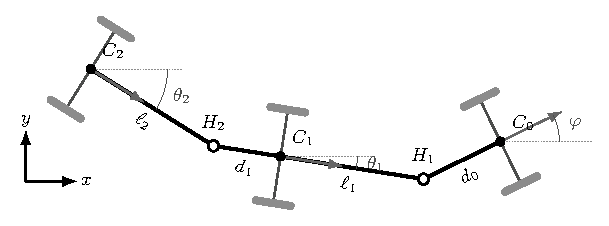
\includegraphics[width=0.85\textwidth]{geometry.pdf}
  \caption{Geometry of the car with two off-hooked trailers. $C_0,C_1,C_2$
  are the axle midpoints, $H_1,H_2$ the hitches, $\varphi,\theta_1,\theta_2$
  the headings measured from the $x$-axis. Proportions are exaggerated for
  legibility.}
  \label{fig:geometry}
\end{figure}

\begin{definition}[Off-hooked trailer]
\label{def:offhooked}
A trailer is \emph{off-hooked} if its hitch is not on the axle of the vehicle in
front of it. In \cref{fig:geometry} this means $\dzero>0$ for the first trailer
and $\done>0$ for the second.
\end{definition}

Off-hooked trailers are harder to control than trailers hitched on the axle.
If $\dzero=\done=0$, the equations can be changed into a simple standard form
called the chained form \cite{sordalen1993}, and there are well-known methods
for controlling it. With off-hooked trailers this is not possible. This is
discussed in Chapter~\ref{ch:background}. What it means for the controller is
explained at the end of \cref{sec:controllability}.

The configuration is collected in the state vector
\begin{equation}
  x=(x_1,x_2,x_3,x_4,x_5)^\top
   =(x_{C_0},\,y_{C_0},\,\varphi,\,\theta_1,\,\theta_2)^\top\in\R^5,
  \label{eq:state}
\end{equation}
where $(x_{C_0},y_{C_0})$ are the coordinates of $C_0$. For an angle $\alpha$, let
$e(\alpha)=(\cos\alpha,\sin\alpha)^\top$ be the unit vector pointing in that
direction. Let $e^\perp(\alpha)=(-\sin\alpha,\cos\alpha)^\top$ be the unit
vector at a right angle to it. Note that $\dot e(\alpha)=\dot\alpha\,e^\perp(\alpha)$.

% ===========================================================================
\section{Rolling-without-slipping constraints}
\label{sec:rolling}

It is assumed that the wheels roll without slipping. This means that a part can
move forward or backward and can turn, but it cannot slide sideways. Take one
part. Let $\alpha$ be the angle it points to, and let $C=(x_C,y_C)$ be the
midpoint of its axle. The sideways direction is $e^\perp(\alpha)$. The sideways
component of the velocity of $C$ is $\dot C\cdot e^\perp(\alpha)$, and it
must be zero:
\begin{equation}
  \dot x_C\sin\alpha-\dot y_C\cos\alpha=0 .
  \label{eq:oneaxle}
\end{equation}

Applied to all three parts, this gives
\begin{align}
  \dot x_{C_0}\sin\varphi-\dot y_{C_0}\cos\varphi&=0,\label{eq:rolling0}\\
  \dot x_{C_1}\sin\theta_1-\dot y_{C_1}\cos\theta_1&=0,\label{eq:rolling1}\\
  \dot x_{C_2}\sin\theta_2-\dot y_{C_2}\cos\theta_2&=0.\label{eq:rolling2}
\end{align}

The state has five numbers, and these are three independent rules that the
motion must follow. So at each moment only two directions of motion are free.
The other three can only be reached by combining the two inputs in sequences of
movements (\cref{sec:controllability}).

% ===========================================================================
\section{Trailer axle positions}
\label{sec:positions}

The first hitch $H_1$ is behind $C_0$, at the distance $\dzero$ in the direction
of the robot: $H_1=C_0-\dzero\,e(\varphi)$. The axle midpoint $C_1$ is a further
$\lone$ behind $H_1$, in the direction of the first trailer. The second hitch
$H_2$ is $\done$ behind $C_1$, in the same direction, and $C_2$ is $\ltwo$ behind
$H_2$, in the direction of the second trailer. This gives
\begin{align}
  C_1&=C_0-\dzero\,e(\varphi)-\lone\,e(\theta_1),\label{eq:C1}\\
  C_2&=C_0-\dzero\,e(\varphi)-(\lone+\done)\,e(\theta_1)-\ltwo\,e(\theta_2).
  \label{eq:C2}
\end{align}
The minus signs mean ``behind'', because $e(\alpha)$ points forward. The lengths
$\lone$ and $\done$ both lie along the first trailer, so in the second equation
they are added together.

% ===========================================================================
\section{Driftless control-affine system}
\label{sec:affine}

The equations of motion follow from the rolling rules. The robot has two
inputs. The first, $u_1$, is how fast it drives forward. The second, $u_2$, is
how fast it turns, in radians per second. The first rolling rule says that the
velocity of $C_0$ points in the direction the robot faces, so
$\dot C_0=u_1\,e(\varphi)$. In coordinates this is
\begin{equation}
  \dot x_1=u_1\cos x_3,\qquad \dot x_2=u_1\sin x_3,\qquad \dot x_3=u_2 .
  \label{eq:robot}
\end{equation}
The first two equations say how the position changes, and the third says that
the angle of the robot changes at the speed $u_2$.

\paragraph{First trailer.}
The first trailer must also not slide sideways. To use this rule, the
velocity of $C_1$ is needed. It is obtained by taking the derivative
of~\eqref{eq:C1}, using $\dot e(\alpha)=\dot\alpha\,e^\perp(\alpha)$:
\begin{equation}
  \dot C_1=\dot C_0-\dzero\,\dot\varphi\,e^\perp(\varphi)
          -\lone\,\dot\theta_1\,e^\perp(\theta_1).
\end{equation}
The rolling rule~\eqref{eq:rolling1} for the first trailer says
$\dot C_1\cdot e^\perp(\theta_1)=0$. The relations $\dot C_0=u_1\,e(\varphi)$ and
$\dot\varphi=u_2$ are put in. Two dot products are also needed:
\begin{equation}
  e(\varphi)\cdot e^\perp(\theta_1)=\sin(\varphi-\theta_1),\qquad
  e^\perp(\varphi)\cdot e^\perp(\theta_1)=\cos(\varphi-\theta_1).
\end{equation}
Then the rule becomes
\begin{equation}
  u_1\sin(\varphi-\theta_1)-\dzero u_2\cos(\varphi-\theta_1)-\lone\dot\theta_1=0.
\end{equation}
Solving for $\dot\theta_1$ gives
\begin{equation}
  \dot x_4=\frac{u_1\sin(x_3-x_4)-\dzero\,u_2\cos(x_3-x_4)}{\lone}.
  \label{eq:x4dot}
\end{equation}
The second term comes from the off-hooked hitch. If $\dzero=0$, the input $u_2$
does not change the trailer angle. If $\dzero>0$, turning the robot on the spot
already pulls the trailer around.

\paragraph{Second trailer.}
The second trailer works in the same way. The derivative
of~\eqref{eq:C2} is
\begin{equation}
  \dot C_2=\dot C_0-\dzero\,\dot\varphi\,e^\perp(\varphi)
          -(\lone+\done)\,\dot\theta_1\,e^\perp(\theta_1)
          -\ltwo\,\dot\theta_2\,e^\perp(\theta_2).
\end{equation}
The rolling rule~\eqref{eq:rolling2} for the second trailer says
$\dot C_2\cdot e^\perp(\theta_2)=0$. The same kind of dot products is needed
as before. The new one is
$e^\perp(\theta_1)\cdot e^\perp(\theta_2)=\cos(\theta_1-\theta_2)$. Then the rule
becomes
\begin{equation}
  u_1\sin(\varphi-\theta_2)-\dzero u_2\cos(\varphi-\theta_2)
  -(\lone+\done)\,\dot\theta_1\cos(\theta_1-\theta_2)-\ltwo\,\dot\theta_2=0 .
\end{equation}
The term with $\dot\theta_1$ is new. It appears because the first trailer pulls
the second one, so when the first trailer turns, it moves the second one too. Solving
for $\dot\theta_2$ and putting in~\eqref{eq:x4dot} gives $\dot x_5$ as a
combination of $u_1$ and $u_2$, with the coefficients $f_{15}$ and $f_{25}$
below.

\paragraph{Result.}
The five equations of motion all have the form ``a function of $x$ times $u_1$,
plus another function of $x$ times $u_2$''. The first functions form the column
$f_1$, and the second functions form the column $f_2$. So the whole system is
\begin{equation}
  \dot x=u_1f_1(x)+u_2f_2(x),\qquad x\in\R^5,\ u\in\R^2,
  \label{eq:system}
\end{equation}
with
\begin{equation}
  f_1(x)=\begin{pmatrix}\cos x_3\\ \sin x_3\\ 0\\
        \dfrac{\sin(x_3-x_4)}{\lone}\\ f_{15}(x)\end{pmatrix},\qquad
  f_2(x)=\begin{pmatrix}0\\ 0\\ 1\\
        -\dfrac{\dzero\cos(x_3-x_4)}{\lone}\\ f_{25}(x)\end{pmatrix},
  \label{eq:fields}
\end{equation}
\begin{align}
  f_{15}(x)&=\frac{\sin(x_3-x_5)}{\ltwo}
     -\frac{(\done+\lone)\sin(x_3-x_4)\cos(x_4-x_5)}{\lone\ltwo},\\
  f_{25}(x)&=\frac{\dzero(\done+\lone)\cos(x_3-x_4)\cos(x_4-x_5)}{\lone\ltwo}
     -\frac{\dzero\cos(x_3-x_5)}{\ltwo}.
\end{align}
A system of this form is called \emph{driftless} and \emph{control-affine}.
Driftless means that nothing moves when $u_1=u_2=0$. Control-affine means that
the inputs only multiply functions of the state, and the results are added.

This system has two important features.

First, $\dot x_3=u_2$ holds exactly: $u_2$ is the turning speed of the robot. A
differential-drive robot can do this directly, so it needs no steering
mechanism. (In~\cite{zuyev2024}, $u_2$ is the steering velocity of a front axle,
but the equations are the same.)

Second, the fourth and fifth entries of $f_2$ are not zero: turning the robot,
without driving forward, moves both trailers. Each of these entries has the
factor $\dzero$, so they would be zero if the hitch were on the axle. The
off-hooked geometry is therefore not a small change to the classical case. It
changes how the inputs reach the trailer angles.

% ===========================================================================
\section{Controllability}
\label{sec:controllability}

The question is whether the system can reach every state near the origin, even
though it has only two inputs. The vector fields $f_1$ and $f_2$ alone do not
answer this, because they give only two directions of motion. The other
directions come from Lie brackets. A Lie bracket describes the motion that is
obtained by combining the two inputs in a sequence (see
Chapter~\ref{ch:background}). The Lie bracket of two vector fields $f_i$ and $f_j$ is
\begin{equation}
  \bracket{f_i}{f_j}(x)=\frac{\partial f_j}{\partial x}(x)\,f_i(x)
                      -\frac{\partial f_i}{\partial x}(x)\,f_j(x).
  \label{eq:bracket}
\end{equation}
(Some books use the opposite sign.) From $f_1$, $f_2$ and their brackets the
matrix
\begin{equation}
  F(x)=\bigl(f_1,\ f_2,\ \bracket{f_1}{f_2},\
     \bracket{f_1}{\bracket{f_1}{f_2}},\
     \bracket{f_1}{\bracket{f_1}{\bracket{f_1}{f_2}}}\bigr)(x)\in\R^{5\times5}
  \label{eq:Fmatrix}
\end{equation}
is built. Its five columns are five directions in which the system can move.

The determinant of $F$ at the origin was computed with a computer algebra
program, with the four lengths kept as symbols. The origin is the straight
configuration, with all angles zero. The result is
\begin{equation}
  \det F(0)=-\frac{(\dzero+\lone)(\dzero+\ltwo)(\done+\ltwo)}
                  {\lone^{4}\,\ltwo^{4}} .
  \label{eq:detF}
\end{equation}
This agrees with~\cite{zuyev2024}. The determinant, the brackets and the growth
vector were also checked with a second script, which derives the model directly
from the rolling rules (Appendix~\ref{app:controllability}).

Every factor in the formula for $\det F(0)$ is positive, because all four
lengths are positive, so $\det F(0)\neq0$. The five columns of $F(0)$ are
therefore linearly independent, and the Lie algebra rank condition holds at the
origin. The determinant is continuous, so the condition also holds in a
neighbourhood of the origin. By the Chow--Rashevskii theorem
\cite{nijmeijer1990}, any two points of this neighbourhood can be joined by an
admissible trajectory. The system~\eqref{eq:system} is therefore controllable
near the origin.

It is also important how many levels of brackets are needed to cover $\R^5$. Let
$\mathcal L^s$ be the set of all directions that can be made from brackets of
$f_1,f_2$ of length at most $s$. The vector fields $f_1,f_2$ have length 1,
$\bracket{f_1}{f_2}$ has length 2, $\bracket{f_1}{\bracket{f_1}{f_2}}$ has
length 3, and so on. Let $n_s$ be the number of independent directions in
$\mathcal L^s$ at the origin. Then
\begin{equation}
  (n_1,n_2,n_3,n_4)=(2,3,4,5).
  \label{eq:growth}
\end{equation}
This list is called the \emph{growth vector}. The smallest $s$ for which $n_s=5$
is the \emph{degree of nonholonomy}. Here it is $r=4$.

In practice, two directions of motion are available immediately: driving and
turning. A third direction needs a manoeuvre that combines both inputs. The
remaining two directions need longer manoeuvres, of length three and four. This
means that the last trailer is the hardest to place. The general meaning of the
growth vector is explained in Chapter~\ref{ch:background}.

This also points to a practical problem. To move in a direction that needs a
long manoeuvre, the inputs have to oscillate with a large amplitude, much larger
than the small movement that results from it. The deeper the direction, the
larger the oscillation. The controller in Chapter~\ref{ch:control} works in this
way. Chapter~\ref{ch:feasibility} shows the consequence: each further level of
brackets makes the time to reach the goal about 100 times longer.

\paragraph{Consequence for feedback.}
Although the system is controllable, no continuous feedback $u=k(x)$ that depends
only on the state can stabilize the origin. The reason is that Brockett's
necessary condition \cite{brockett1983} (Chapter~\ref{ch:background}) is not
satisfied. The first three components of $f(x,u)=u_1f_1(x)+u_2f_2(x)$ are
$(u_1\cos x_3,\,u_1\sin x_3,\,u_2)$. A velocity such as
$(0,0,0,0,\varepsilon)^\top$ with $\varepsilon\neq0$ would need $u_1=u_2=0$, and
then $f=0$. So this velocity can never be produced, however close the system is
to the goal and however small the inputs are. The set of velocities that the
system can produce therefore misses a whole direction. A stabilizing controller
must depend on time. This is the subject of Chapters~\ref{ch:nilpotent}
and~\ref{ch:control}.

% ===========================================================================
\section{Reduction to one trailer}
\label{sec:onetrailer}

The first four components of $f_1$ and $f_2$ do not contain $x_5$, $\done$ or
$\ltwo$. So if the second trailer is removed, the remaining system has the state
$x=(x_1,x_2,x_3,x_4)^\top\in\R^4$, and it is again driftless and
control-affine. Its vector fields $\bar f_1$ and $\bar f_2$ are the first four
components of $f_1$ and $f_2$:
\begin{equation}
  \dot x=u_1\bar f_1(x)+u_2\bar f_2(x),\qquad
  \bar f_1=\begin{pmatrix}\cos x_3\\ \sin x_3\\ 0\\ \dfrac{\sin(x_3-x_4)}{\lone}\end{pmatrix},\quad
  \bar f_2=\begin{pmatrix}0\\ 0\\ 1\\ -\dfrac{\dzero\cos(x_3-x_4)}{\lone}\end{pmatrix}.
  \label{eq:onetrailer}
\end{equation}
The first two brackets of the one-trailer system can be computed in closed form:
\begin{align}
  \bracket{\bar f_1}{\bar f_2}&=\Bigl(\sin x_3,\ -\cos x_3,\ 0,\
        -\frac{\dzero+\lone\cos(x_3-x_4)}{\lone^{2}}\Bigr)^{\!\top},\\
  \bracket{\bar f_1}{\bracket{\bar f_1}{\bar f_2}}&=\Bigl(0,\ 0,\ 0,\
        -\frac{\dzero\cos(x_3-x_4)+\lone}{\lone^{3}}\Bigr)^{\!\top}.
\end{align}
The matrix $\bar F=(\bar f_1,\ \bar f_2,\ \bracket{\bar f_1}{\bar f_2},\ \bracket{\bar f_1}{\bracket{\bar f_1}{\bar f_2}})$
has the determinant
\begin{equation}
  \det\bar F(x)=-\frac{\dzero\cos(x_3-x_4)+\lone}{\lone^{3}},\qquad
  \det\bar F(0)=-\frac{\dzero+\lone}{\lone^{3}}\neq0 .
\end{equation}
Since $\det\bar F(0)\neq0$, the one-trailer system is also controllable near the
origin. Its growth vector is
\begin{equation}
  (n_1,n_2,n_3)=(2,3,4),
\end{equation}
so its degree of nonholonomy at the origin is $r=3$. With one trailer, the
longest manoeuvre that is needed is shorter: three instead of four. As the
following chapters show, this makes the control problem much easier
(\cref{sec:feas-r} compares the two systems). The one-trailer system is
therefore treated together with the two-trailer system throughout the thesis.
The controller is designed for both (Chapters~\ref{ch:control}
and~\ref{ch:feasibility}), both are simulated (Chapter~\ref{ch:simulation}), and
the one-trailer system is the first candidate for experiments
(Chapter~\ref{ch:experiments}).

The determinant $\det\bar F(x)$ is zero where $\dzero\cos(x_3-x_4)=-\lone$. This
can happen only if $\dzero>\lone$, at the angle
$|x_3-x_4|=\arccos(-\lone/\dzero)$ between the robot and the trailer. For the
measured lengths (\cref{sec:parameters}), this angle is about $2.36\,\mathrm{rad}$
($135^\circ$). This concerns only the matrix $\bar F$, and not the rank of the
whole Lie algebra. It is not needed in what follows.
\TODO[measure the largest angle of the first hitch (about 70 degrees?) and say here whether 135 degrees can be reached]

% ===========================================================================
\section{Physical parameters of the platform}
\label{sec:parameters}

The platform used in the simulations and in the experiments is a TurtleBot3
Burger that pulls two printed trailers. The four lengths from \cref{sec:geometry}
were measured on the assembled hardware. The whole train was lying straight
against a straight edge, with all joint angles equal to zero. Each length was
measured along the centre line of the train, which is a straight line through
the middle of all three parts. It goes from one axle or hitch pin to the next
(\cref{tab:geometry-values}).

\begin{table}[ht]
  \centering
  \caption{Measured lengths of the platform.}
  \label{tab:geometry-values}
  \begin{tabular}{llr}
    \toprule
    length & from -- to & value [mm]\\
    \midrule
    $\dzero$ & axle of the robot -- first hitch & 115\\
    $\lone$  & first hitch -- axle of trailer 1 & 82\\
    $\done$  & axle of trailer 1 -- second hitch & 84\\
    $\ltwo$  & second hitch -- axle of trailer 2 & 89\\
    \bottomrule
  \end{tabular}
\end{table}

Two features of these numbers matter later. First, the train is strongly
off-hooked: $\dzero/\lone=1.40$ and $\done/\ltwo=0.94$, so that the first hitch lies
farther behind the axle of the robot than the axle of the trailer lies behind
the hitch. Second, the two tail joints are not identical, so $\dzero$
and $\done$ were measured separately. The results for the platform use the measured values.
\TODO[error of the four lengths (measuring tool and estimated error), play in the joints, masses, wheel diameter and track width are not yet recorded in the thesis; see the measurement sheet]

% ---------------------------------------------------------------------------
% Chapter -- Nilpotent Approximation
%
% DRAFT 1 (19 Oct 2026). Proposed by Claude, to be read and rewritten in
% your own words. Every formula in this chapter was re-derived with sympy
% (code/verify_nilpotent.py) and agrees with the MATLAB code
% (one_trailer_coeff, offhooked_coeffs, x_to_z) and with
% Zuyev & Grushkovskaya, arXiv:2403.03341, Sec. III.
% The one-trailer derivation (Sec. 4.4) is your own, not in the paper.
% ---------------------------------------------------------------------------

\chapter{Nilpotent Approximation}
\label{ch:nilpotent}
\TODO[status of this chapter: about 80 percent done]

The model from Chapter~\ref{ch:model} is controllable, but its equations
contain sines and cosines. Also, no continuous feedback that depends only on the
state can stabilize it. The controllers in Chapter~\ref{ch:control} are
therefore designed for a simpler system. This system keeps only the terms that
matter most for small motions near the origin. It is called the nilpotent
approximation. This chapter explains what it is and why it is used. It is
derived for the car with one trailer (\cref{sec:approx1}) and, following
\cite{zuyev2024}, for two trailers (\cref{sec:approx2}).

% ===========================================================================
\section{Why linearization is not enough}
\label{sec:linearization}

The first idea is to linearize the system, that is, to replace it near the
origin by a linear system. The system has no drift, so the origin with zero
inputs is an equilibrium. The linearization is
\begin{equation}
  \dot x=f_1(0)\,u_1+f_2(0)\,u_2 .
  \label{eq:linearization}
\end{equation}
This system can only move in the plane spanned by $f_1(0)$ and $f_2(0)$, but the
state has five numbers (four for one trailer). So the linearization is not
controllable. It keeps the two directions that are available at once and drops
all the others. These others come from the Lie brackets, and they are exactly
the directions in which the original system is controllable
(\cref{sec:controllability}).

The fix is to look at each direction on its own scale. Suppose the inputs are
of size one and are used for a short time $\varepsilon$. Then the robot moves
about $\varepsilon$ in the first two directions, driving and turning. In a
direction that needs a manoeuvre of length $s$, it moves only about
$\varepsilon^{s}$, which is much less. So the directions cannot be measured on
the same scale. This is made exact by weights (\cref{sec:privileged}).

% ===========================================================================
\section{Privileged coordinates and weights}
\label{sec:privileged}

The construction comes from Bella\"iche, Jean and Risler~\cite{bellaiche2005},
in the form used in~\cite{zuyev2024}. It starts from the directions
$\mathcal L^s(0)$ of \cref{sec:controllability}. These are the directions at the
origin that can be made from brackets of length at most $s$, and there are $n_s$
of them. Each longer bracket adds more directions, until all of $\R^n$ is
covered. This is possible because the Lie algebra rank condition holds at the
origin. The result is a chain of spaces, each inside the next, which is called a
flag:
\begin{equation}
  \{0\}\subset\mathcal L^1(0)\subset\dots\subset\mathcal L^r(0)=\R^n ,
  \qquad \dim\mathcal L^s(0)=n_s .
\end{equation}

\paragraph{Weights.}
Every coordinate $y_j$ gets a weight. The weight is the smallest $s$ for which
some direction in $\mathcal L^s(0)$ changes $y_j$. In other words, $y_j$ has
weight $s$ if it is first reached by manoeuvres of length $s$. For the growth
vector $(2,3,4,5)$ from \eqref{eq:growth}, the weights are
\begin{equation}
  w=(1,1,2,3,4).
  \label{eq:weights}
\end{equation}
The first two coordinates have weight 1, because two directions are available at
once. The other three have weights 2, 3 and 4. For one trailer, with growth
vector $(2,3,4)$, the weights are $w=(1,1,2,3)$. In general, $w_j$ is the
smallest $s$ with $n_s\ge j$.

\paragraph{Linear step.}
Take the vectors $Y_1=f_1$, $Y_2=f_2$, $Y_3=[f_1,f_2]$, $Y_4=[f_1,[f_1,f_2]]$,
and so on. They are the columns of the matrix $F$ from \eqref{eq:Fmatrix}. At the
origin they are independent, so they can be used as new axes. The new
coordinates are
\begin{equation}
  y=F(0)^{-1}x .
  \label{eq:ylinear}
\end{equation}
The number $y_j$ says how much of the direction $Y_j(0)$ the state contains. The
vector $Y_j$ is made from brackets of length $w_j$, and so the coordinate $y_j$
has the weight $w_j$.

\paragraph{Nonlinear correction.}
The coordinates $y$ are not always good enough. The new coordinates have to be
\emph{privileged}, which means that a coordinate with weight $w_j$ changes at
most about $\varepsilon^{w_j}$ when the inputs are used for a short time
$\varepsilon$ \cite{bellaiche2005}. The coordinates $y$ do not always do this,
so they are corrected. The correction is given by the recursion
\begin{equation}
  z_q=y_q-\sum_{(\alpha,w)<w_q}\frac{1}{\alpha_1!\cdots\alpha_{q-1}!}
      \bigl(Y_1^{\alpha_1}\cdots Y_{q-1}^{\alpha_{q-1}}y_q\bigr)(0)\,
      z_1^{\alpha_1}\cdots z_{q-1}^{\alpha_{q-1}},
  \label{eq:bellaiche}
\end{equation}
where $(\alpha,w)=\sum_i w_i\alpha_i$. The recursion subtracts from $y_q$ all
terms whose weighted degree is smaller than $w_q$. For the systems in this thesis
almost all of these terms are zero. The details are in \cref{sec:approx1} and
\cref{sec:approx2}.

\paragraph{A practical test.}
Whether the coordinates are privileged can be checked on the equations. In the
exact equation for $\dot z_q$, every $z_i$ is replaced by $\varepsilon^{w_i}z_i$,
and the result is expanded in $\varepsilon$. A coordinate with weight $w_q$
changes by about $\varepsilon^{w_q}$ during a time $\varepsilon$, so its speed
$\dot z_q$ should be of size $\varepsilon^{w_q-1}$. This means that the lowest
power of $\varepsilon$ must be exactly $w_q-1$. The coefficient of this power is
the $q$-th component of the approximating system. If the lowest power is smaller,
the coordinate moves faster than its weight allows, and it needs a correction.
As an example, take $z_3=-x_2$ and $z_2=x_3$. Then
\begin{equation}
  \dot z_3=-u_1\sin x_3=-u_1\sin z_2
  \;\xrightarrow{\;z_2\to\varepsilon z_2\;}\;
  -\varepsilon\,u_1z_2+O(\varepsilon^3).
\end{equation}
The lowest power is $\varepsilon^1=\varepsilon^{w_3-1}$, because $w_3=2$. All
coordinates in this thesis were checked in this way
(\cref{app:nilpotent}).

% ===========================================================================
\section{Quasi-homogeneity}
\label{sec:homogeneity}

The weights tell how to stretch the coordinates. For a number $\lambda>0$, the
stretching is
\begin{equation}
  \delta_\lambda(z_1,\dots,z_n)=(\lambda^{w_1}z_1,\dots,\lambda^{w_n}z_n).
\end{equation}
Every coordinate is stretched by the power of $\lambda$ given by its weight. This
is the same idea as in \cref{sec:linearization}, where a short time $\varepsilon$
changes a coordinate with weight $w$ by about $\varepsilon^{w}$. The weights also
give a \emph{weighted degree} to every term. A term
$z_1^{\alpha_1}\cdots z_n^{\alpha_n}$ has the degree $\sum_iw_i\alpha_i$. For
example, $z_3$ and $z_2^2$ both have degree $2$, and $z_4$ and $z_2^3$ both have
degree $3$.

A vector field $X$ has one component $X_j$ for each coordinate. It is
\emph{weighted homogeneous of degree $m$} if every component $X_j$ has weighted
degree $w_j+m$, which means that all its terms have this degree. The fields of
the nilpotent approximation, which is derived below, have degree $-1$: the
component $j$ has degree $w_j-1$. This is what the practical test in
\cref{sec:privileged} checks. It has three consequences, and they show why the
approximation is useful.

\begin{enumerate}
  \item The bracket of two weighted homogeneous fields with degrees $m$ and $m'$
        is weighted homogeneous of degree $m+m'$. Let $g_1$ and $g_2$ be the two
        fields of the nilpotent approximation. Both have degree $-1$, so a
        bracket of length $k$ of $g_1$ and $g_2$ has degree $-k$.
  \item The fields $g_1$ and $g_2$ are polynomial, which means that their
        components are polynomials in $z$. A bracket of length $k$ has degree
        $-k$, so its component $j$ has degree $w_j-k$. A polynomial cannot have
        a negative degree, so this component is zero when $w_j<k$. Therefore all
        brackets of length greater than $r=\max_jw_j$ are zero. A Lie algebra
        with this property is called \emph{nilpotent} (of step $r$), and this is
        where the name of the approximation comes from. The exact system is not
        nilpotent, because its sines and cosines produce new terms at every
        length.
  \item A component of degree $w_j-1$ can contain only coordinates with a smaller
        weight than $w_j$. So $\dot z_j$ depends only on $z_1,\dots,z_{j-1}$, and
        the system is triangular. A triangular system can be solved one
        coordinate after the other, with a formula. The controller of
        Chapter~\ref{ch:control} uses this.
\end{enumerate}

In privileged coordinates, the exact system differs from the approximating
system only by terms of higher weighted degree~\cite{bellaiche2005}. Close to the
origin, these terms are small compared with the terms of the approximation. A
controller designed for the nilpotent approximation can therefore be expected to
work for the exact system too, as long as the difference stays small.
Chapter~\ref{ch:control} shows how this is made exact.
Chapter~\ref{ch:simulation} measures the size of the difference. There, the
controller is simulated on the approximation and on the exact kinematics, and the
two results are compared (\cref{sec:sim-exact,sec:sim-validity}).

% ===========================================================================
\section{Approximation for one trailer}
\label{sec:approx1}

In this section, the construction is carried out for the car with one off-hooked
trailer, that is, for the system with four coordinates from
\eqref{eq:onetrailer}. Its weights are $w=(1,1,2,3)$ and its degree of
nonholonomy is $r=3$. The paper~\cite{zuyev2024} treats only two trailers, so this
derivation is not in it.

\paragraph{Privileged coordinates.}
For one trailer, the matrix $F(0)$ is made of $\bar f_1$, $\bar f_2$ and their
brackets from \cref{sec:onetrailer}. It is
\begin{equation}
  F(0)=\begin{pmatrix}
    1&0&0&0\\
    0&0&-1&0\\
    0&1&0&0\\
    0&-\dfrac{\dzero}{\lone}&-\dfrac{\dzero+\lone}{\lone^{2}}&-\dfrac{\dzero+\lone}{\lone^{3}}
  \end{pmatrix}.
\end{equation}
The linear step \eqref{eq:ylinear} gives the new coordinates
\begin{equation}
  z_1=x_1,\qquad z_2=x_3,\qquad z_3=-x_2,\qquad
  z_4=\lone x_2-\frac{\dzero\lone^{2}}{\dzero+\lone}\,x_3
      -\frac{\lone^{3}}{\dzero+\lone}\,x_4 .
  \label{eq:xtoz1}
\end{equation}
They are found by writing $x$ as a mix of the four directions
$Y_1(0),\dots,Y_4(0)$ and solving for the amounts. They are called $z$, because
no nonlinear correction is needed, as shown below. The inverse map is
$x=F(0)z$, and it is used to plot the motion in the original coordinates. It
reads $x_1=z_1$, $x_2=-z_3$, $x_3=z_2$ and
$x_4=-\frac{\dzero}{\lone}z_2-\frac{\dzero+\lone}{\lone^{2}}z_3
-\frac{\dzero+\lone}{\lone^{3}}z_4$.
Only the state is written in new coordinates. The inputs $u_1$ and $u_2$ are the
physical velocities in both descriptions.

\paragraph{No nonlinear correction is needed.}
The correction \eqref{eq:bellaiche} subtracts only terms of weighted degree
smaller than $w_q$. The highest weight here is $w_4=3$, so a cubic term such as
$z_2^3$ (degree $3$) is never subtracted. In the two-trailer system it is,
because there $w_5=4>3$. Terms of degree $2$, which is less than $3$, could be
subtracted in principle, but they are not needed. The practical test below finds
no power of $\varepsilon$ below $w_q-1$. So the coordinates from the linear step
are already privileged.

\paragraph{Equations in the new coordinates.}
The first three equations follow from \eqref{eq:robot}:
$\dot z_1=u_1\cos z_2$, $\dot z_2=u_2$, $\dot z_3=-u_1\sin z_2$.
For $z_4$, the derivative of \eqref{eq:xtoz1} is computed, and $\dot x_2$,
$\dot x_3$ and $\dot x_4$ are taken from the system, using \eqref{eq:x4dot}.
This gives the exact expression
\begin{equation}
  \dot z_4=u_1\,\lone\Bigl[\sin x_3-\frac{\lone}{\dzero+\lone}\sin(x_3-x_4)\Bigr]
  -u_2\,\frac{\dzero\lone^{2}}{\dzero+\lone}\bigl[1-\cos(x_3-x_4)\bigr].
  \label{eq:z4dot}
\end{equation}
Here $x_3$ and $x_4$ have to be replaced by their expressions in $z$. From the
inverse map,
\begin{equation}
  x_3-x_4=\frac{\dzero+\lone}{\lone}\,z_2+\frac{\dzero+\lone}{\lone^{2}}\,z_3
          +\frac{\dzero+\lone}{\lone^{3}}\,z_4 .
\end{equation}
Next, every $z_i$ is replaced by $\varepsilon^{w_i}z_i$, and the result is
expanded in $\varepsilon$, as in the practical test of \cref{sec:privileged}. In
the $u_1$ term, the parts of order $\varepsilon^1$ cancel, because
$\lone\bigl[z_2-\frac{\lone}{\dzero+\lone}\cdot\frac{\dzero+\lone}{\lone}z_2\bigr]=0$.
The part of order $\varepsilon^2$ is $-z_3$. In the $u_2$ term,
$1-\cos(x_3-x_4)=\tfrac12\bigl(\tfrac{\dzero+\lone}{\lone}z_2\bigr)^2\varepsilon^2
+O(\varepsilon^3)$. Altogether
\begin{equation}
  \dot z_4=\varepsilon^2\bigl(-z_3u_1-\alpha z_2^2u_2\bigr)+O(\varepsilon^3),
  \qquad
  \alpha=\frac{\dzero(\dzero+\lone)}{2}.
  \label{eq:alpha1}
\end{equation}
The powers $\varepsilon^0$ and $\varepsilon^1$ vanish, and the lowest power is
$\varepsilon^2=\varepsilon^{w_4-1}$, as required.

\paragraph{The approximating system.}
In each equation, only the term with the lowest power of $\varepsilon$ is kept,
and $\varepsilon$ is set to $1$. This gives the nilpotent approximation for one
trailer:
\begin{equation}
  \dot z=u_1g_1(z)+u_2g_2(z),\qquad
  g_1(z)=\begin{pmatrix}1\\0\\-z_2\\-z_3\end{pmatrix},\quad
  g_2(z)=\begin{pmatrix}0\\1\\0\\-\alpha z_2^{2}\end{pmatrix}.
  \label{eq:nilp1}
\end{equation}
It has only one parameter, $\alpha$. So the system depends on the geometry only
through $\dzero$ and $\lone$, and $\alpha>0$ for all positive $\dzero$ and
$\lone$. For the platform values $\dzero=\SI{0.115}{m}$ and
$\lone=\SI{0.082}{m}$ (\cref{sec:parameters}), $\alpha\approx\SI{1.133e-2}{m^2}$.

\paragraph{Brackets and the matrix $G$.}
The brackets of the approximating fields are constant:
\begin{equation}
  [g_1,g_2]=(0,0,1,0)^\top,\qquad
  [g_1,[g_1,g_2]]=(0,0,0,1)^\top .
\end{equation}
Also, $[g_2,[g_1,g_2]]=0$, and all brackets of length four are zero. So the Lie
algebra is nilpotent of step three, as predicted in \cref{sec:homogeneity}.
The matrix $G(z)$ has the columns $g_1$, $g_2$, $[g_1,g_2]$ and
$[g_1,[g_1,g_2]]$. It is lower triangular with ones on the diagonal, so
\begin{equation}
  \det G(z)=1\qquad\text{for all }z .
  \label{eq:detG}
\end{equation}
This is different from \cref{sec:controllability}, where $\det F(0)\ne0$ was a
condition that had to be checked for the real system. Here, $\det G=1$ holds for
every system of this triangular form. It only confirms that the construction was
carried out correctly. It also means that the inverse $G(z)^{-1}$ exists for
every $z$. The controller of Chapter~\ref{ch:control} uses this inverse, so it is
well defined everywhere.

\paragraph{The chained form appears by itself.}
If $\dzero\to0$, which means that the hitch is on the axle, then $\alpha\to0$ and
\begin{equation}
  \dot z_4=-z_3u_1 .
\end{equation}
This is exactly the chained form from~\cite{sordalen1993}. The chained form was
not used anywhere in the derivation, and it comes out by itself in this case.
When the hitch is off the axle, the term $-\alpha z_2^2u_2$ is the only
difference from the classical case. This agrees with the discussion in
\cref{sec:geometry}.

% ===========================================================================
\section{Approximation for two trailers}
\label{sec:approx2}

The approximation for the car with two trailers was obtained
in~\cite{zuyev2024}. It is summarized here, together with the checks made for
this thesis.

The weights are $w=(1,1,2,3,4)$. The linear coordinates $y=F(0)^{-1}x$ are given
in~\cite{zuyev2024}, and their entries are fractions made of the four lengths.
For two trailers, the correction \eqref{eq:bellaiche} is not zero. The only term
that survives is cubic in $x_3=z_2$, and its degree is $3<w_5=4$. So
\begin{equation}
  z_1=x_1,\quad z_2=x_3,\quad z_3=-x_2,\quad z_4=y_4,\quad
  z_5=y_5-\beta x_3^{3},
  \label{eq:xtoz2}
\end{equation}
with
\begin{equation}
  \beta=\frac{\dzero\ltwo\bigl[\dzero^{2}(\done+\lone)(\lone-\ltwo-\done)
        +\lone^{3}(\dzero+\ltwo)\bigr]}{6(\dzero+\ltwo)\lone^{2}} .
\end{equation}
The coefficient $\beta$ is chosen so that it cancels the term of order
$\varepsilon^2$ in $\dot z_5$. Without it, this term would fail the practical test
of \cref{sec:privileged}.

The approximating system is
\begin{equation}
  \dot z_1=u_1,\quad \dot z_2=u_2,\quad \dot z_3=-z_2u_1,\quad
  \dot z_4=-z_3u_1-\alpha z_2^{2}u_2,\quad
  \dot z_5=(\kappa z_2^{3}-z_4)u_1-\theta z_2z_3u_2 ,
  \label{eq:nilp2}
\end{equation}
That is, $g_1=(1,0,-z_2,-z_3,\kappa z_2^3-z_4)^\top$ and
$g_2=(0,1,0,-\alpha z_2^2,-\theta z_2z_3)^\top$. The coefficients are
\begin{align}
  \alpha&=\frac{\dzero^{3}\bigl[\lone^{3}+\lone^{2}\ltwo-\lone\ltwo^{2}-\done\ltwo(\done+\ltwo)\bigr]
         +\dzero\lone^{3}\bigl[\dzero(\lone+2\ltwo)+\ltwo(\lone+\ltwo)\bigr]}
         {2(\dzero+\ltwo)\lone^{3}},\\[2pt]
  \kappa&=\frac{\dzero^{2}\Bigl\{\tfrac32\ltwo^{2}(\dzero+\lone)(\done+\lone)
         -\ltwo\bigl[\lone^{3}+\tfrac12\dzero\lone^{2}-\done\lone(\dzero+\tfrac32\done)
         -\tfrac32\dzero\done^{2}\bigr]+\tfrac12\dzero\done^{2}\lone\Bigr\}}
         {3(\dzero+\ltwo)\lone^{3}},\\[2pt]
  \theta&=\frac{\dzero^{2}\bigl[\ltwo^{2}(\done+\lone)(\dzero+\lone)
         +\bigl(\dzero\done+(\dzero+\done)\lone\bigr)\done\ltwo+\dzero\done^{2}\lone\bigr]}
         {(\dzero+\ltwo)\lone^{3}} .
\end{align}
The symbol $\alpha$ is used again, but it is not the same number as for one
trailer, because $z_4$ is defined differently here.

As a check, the two parameter sets of the numerical example in
\cite{zuyev2024} ($\dzero=\done=0.1$, $\lone=\ltwo=1$ and
$\dzero=\done=\lone=\ltwo=1$) give $(\alpha,\kappa,\theta)=(0.10495,\,0.0024,\,0.0112)$
and $(1,\,1.5,\,4)$ with these formulas. These are the values printed in the
paper. They were also checked with the MATLAB function
\texttt{offhooked\_coeffs} (Chapter~\ref{ch:feasibility}) and with a symbolic
computation (\cref{app:nilpotent}).
\TODO[the denominator of alpha in eq. (11) of the paper seems to contain $\ell_2^3$, but the derivation here gives $\ell_1^3$; the examples cannot tell because $\ell_1=\ell_2$ there; check the PDF]

The matrix $G(z)$ has the columns $g_1$, $g_2$ and the brackets up to length
four. It is again lower triangular with ones on the diagonal, so
$\det G(z)=1$. Its third column, the bracket $[g_1,g_2]$, is
$(0,0,1,0,-(\alpha+3\kappa-\theta)z_2^{2})^\top$.

Compare the approximations for one and two trailers, \eqref{eq:nilp1} and
\eqref{eq:nilp2}. The first four equations have the same form. The coefficient
$\alpha$ is different, because $z_4$ is defined differently in the two cases: for
two trailers, $y_4$ contains $x_5$. The second trailer adds one equation and a
correction $\beta$, and it gives three coefficients instead of one. It also
raises the weight of the last coordinate from $3$ to $4$.

\begin{table}[t]
  \centering
  \caption{Nilpotent approximation of the car with one and two trailers.}
  \label{tab:approx}
  \begin{tabular}{lcc}
    \toprule
                                   & one trailer & two trailers \\
    \midrule
    state dimension                & 4           & 5 \\
    growth vector                  & $(2,3,4)$   & $(2,3,4,5)$ \\
    weights                        & $(1,1,2,3)$ & $(1,1,2,3,4)$ \\
    degree of nonholonomy $r$      & 3           & 4 \\
    nonlinear correction           & none        & $\beta$ (cubic term in $z_5$) \\
    coefficients                   & $\alpha$    & $\alpha,\kappa,\theta$ \\
    $\det G(z)$                    & 1           & 1 \\
    \bottomrule
  \end{tabular}
\end{table}

% ===========================================================================
\section{Verification}
\label{sec:verification}

The derivation in \cref{sec:approx1} is not copied from a paper, so it was
checked in four ways.

\begin{enumerate}
  \item \textbf{$\det G(z)=1$.} The matrix of brackets of the approximating system
        has determinant $1$ for all $z$, for one and for two trailers. This only
        confirms that the matrix is triangular with ones on the diagonal, as the
        construction should give.
  \item \textbf{Nilpotency.} All brackets of length greater than $r$ are zero
        ($r=3$ and $r=4$), as predicted in \cref{sec:homogeneity}.
  \item \textbf{The limit $\dzero\to0$ gives the chained form.} This is a strong
        check, because the chained form was not used in the construction. It is
        a known fact from the classical theory, and the derivation reproduces it.
  \item \textbf{Symbolic computation.} The practical test of
        \cref{sec:privileged} was applied symbolically (\cref{app:nilpotent}).
        For one trailer, with $\dzero$ and $\lone$ left as symbols, it gives
        $\alpha=\dzero(\dzero+\lone)/2$. For two trailers, it determines $\beta$
        from the requirement that the $\varepsilon^2$ term of $\dot z_5$ is zero.
        It also reproduces $\alpha,\kappa,\theta,\beta$ of this chapter exactly,
        as fractions, for three sets of lengths. These are the two sets quoted in
        \cite{zuyev2024}, one of them giving $\alpha=0.10495$, $\kappa=0.0024$,
        $\theta=0.0112$, and the platform lengths.
\end{enumerate}
A general MATLAB routine, \texttt{derive\_privileged.m}, gives the same results.
It receives only the fields $f_1$ and $f_2$, and it finds the weights, the
correction and the approximating system by itself. For two trailers, it
reproduces the coefficient $\beta$ of~\cite{zuyev2024} exactly.

\paragraph{What is not verified.}
The nilpotent approximation keeps only the leading terms, so it is not exact. How
close a controller designed for it comes to the exact kinematics of
Chapter~\ref{ch:model} is measured by simulation in
Chapter~\ref{ch:simulation} (\cref{sec:sim-exact,sec:sim-validity}).

% ---------------------------------------------------------------------------
% Chapter -- Oscillating Control Design
% The controller is the r = 3 truncation of eq. (16) of
% Zuyev & Grushkovskaya, arXiv:2403.03341, Sec. IV.
% The paper proves convergence for r = 4 only (see Section 5.5).
% Figure: code/fig_one_period.py -> figures/fig_one_period.pdf
% ---------------------------------------------------------------------------

\chapter{Oscillating Control Design}
\label{ch:control}
\TODO[status of this chapter: text rewritten; two open questions for the supervisor, see the TODOs in 5.4 and 5.5]

Chapter~\ref{ch:model} showed that no continuous feedback that depends only on
the state can stabilize the car with trailers. Chapter~\ref{ch:nilpotent}
replaced the model by a simpler system, the nilpotent approximation
$\dot z=u_1g_1(z)+u_2g_2(z)$. This chapter designs a controller for that system,
and the controller depends on time. The approach comes
from~\cite{zuyev2016,grushkovskaya2023}, and it was applied to off-hooked
trailers in~\cite{zuyev2024}. The inputs oscillate, and the oscillations move
the system in the directions that the two inputs cannot reach directly. For the
car with one trailer, the controller is a shortened version of the controller
from~\cite{zuyev2024}: it is cut after the second bracket ($r=3$).
\Cref{sec:convergence} says what is proved for it and what is not.

% ===========================================================================
\section{Idea}
\label{sec:idea}

Take the nilpotent system $\dot z=u_1g_1(z)+u_2g_2(z)$ with the matrix $G(z)$
from \cref{sec:approx1}. Suppose that all four coordinates could be moved
independently. This would mean a ``virtual'' input $v$ with four components, so
that $\dot z=G(z)v$, and $v$ could be chosen so that $z$ moves toward the goal.
The real system has only two inputs. But the oscillating inputs defined below
give, over one period $\varepsilon$, the displacement
\begin{equation}
  z(\varepsilon)\approx z(0)+\varepsilon\,G(z)\,a(z),
  \label{eq:step}
\end{equation}
where $a=(a_1,a_2,a_{12},a_{112})^\top$ is a vector of four amplitudes that can
be chosen freely. The amplitudes $a_1$ and $a_2$ move the coordinates that are
reached directly. The amplitudes $a_{12}$ and $a_{112}$ move the coordinates that
are reached through the first and the second Lie bracket. This is why the indices
are the brackets written as digits. The formula is made exact in
\cref{sec:convergence}.

Next, a function $V(z)$ is chosen that measures how far $z$ is from the goal. It
is zero at the goal and positive everywhere else. It is called a Lyapunov
function. The amplitudes are chosen as
\begin{equation}
  a(z)=-G(z)^{-1}\nabla V(z).
  \label{eq:agradient}
\end{equation}
Then $G(z)a(z)=-\nabla V(z)$, and \eqref{eq:step} becomes
\begin{equation}
  z_{j+1}\approx z_j-\varepsilon\nabla V(z_j).
\end{equation}
This is one step of gradient descent with step length $\varepsilon$: the state
moves a little in the direction in which $V$ decreases fastest. For small steps,
this is the gradient flow $\dot z=-\nabla V(z)$. This is the core of the method:
\emph{one period of the oscillating controller is one step of gradient descent
in the privileged coordinates.} The inverse $G(z)^{-1}$ exists for every $z$,
because $\det G(z)=1$ \eqref{eq:detG}, so this choice is always possible.

\paragraph{Radial Lyapunov functions.}
In this thesis, $V$ depends only on the distance $r=\|z\|$ to the goal:
$V(z)=\Phi(r)$. Then $\nabla V(z)=(\Phi'(r)/r)\,z$. It is convenient to write this
as $\nabla V(z)=\gamma\,h(z)\,z$, so that
\begin{equation}
  a(z)=-\gamma\,h(z)\,G(z)^{-1}z,\qquad h(z)=\frac{\Phi'(r)}{\gamma r}.
  \label{eq:ah}
\end{equation}
The constant $\gamma>0$ is called the gain. The function $h$ is the only place
where the choice of $V$ enters the controller. Three choices are used:
\begin{center}
\begin{tabular}{lll}
  \toprule
  $V$ & $\Phi(r)$ & $h(z)$ \\
  \midrule
  quadratic & $\gamma r^2/2$ & $1$ \\
  logarithmic & $\dfrac{\gamma}{2c}\ln(1+cr^2)$ & $\dfrac{1}{1+c\,r^2}$ \\[6pt]
  square-root & $\gamma\bigl(\sqrt{r^2+\delta^2}-\delta\bigr)$ & $\dfrac{1}{\sqrt{r^2+\delta^2}}$ \\
  \bottomrule
\end{tabular}
\end{center}
They differ in how the length of the step depends on the distance to the goal.
Their effect on the speed of convergence is compared in
Chapter~\ref{ch:feasibility}.
For the car with one trailer, $G(z)$ is lower triangular, and \eqref{eq:ah}
gives
\begin{equation}
  \begin{aligned}
  a_1&=-\gamma h\,z_1, & a_{12}&=-\gamma h\,(z_1z_2+z_3),\\
  a_2&=-\gamma h\,z_2, & a_{112}&=-\gamma h\,(\alpha z_2^{3}+z_1z_3+z_4).
  \end{aligned}
  \label{eq:amps}
\end{equation}
Each amplitude is large when the coordinate it belongs to is far from zero. The
extra terms, such as $z_1z_2$ in $a_{12}$, are needed because the directions
$g_1,g_2,\dots$ influence each other's coordinates. For example, moving $z_1$ and
$z_2$ also changes $z_3$.

\begin{figure}[t]
  \centering
  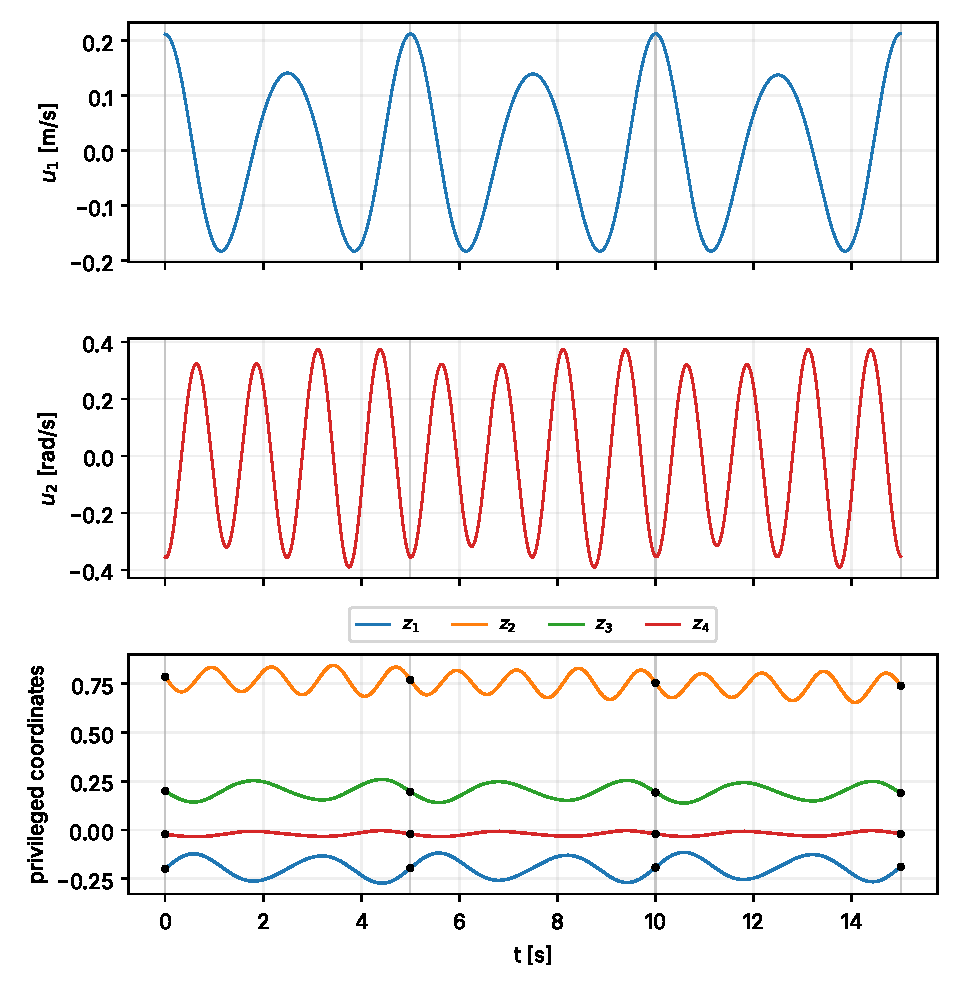
\includegraphics[width=0.78\textwidth]{fig_one_period.pdf}
  \caption{The controller over three sampling intervals (one trailer, platform
  lengths, $\varepsilon=\SI{5}{s}$, $(k_{12},k_{112})=(3,2)$,
  $\|z(0)\|=0.835$). Top and middle: the inputs $u_1$ and $u_2$. Bottom: the
  privileged coordinates. The dots mark the start of each interval. Within an
  interval, the coordinates swing back and forth. Over a full period, the net
  movement is the small gradient step \eqref{eq:step}.}
  \label{fig:oneperiod}
\end{figure}

% ===========================================================================
\section{Controller structure}
\label{sec:structure}

The controller has a constant part and one oscillating term for each level of
Lie brackets. Let $\omega=2\pi/\varepsilon$. For $r=3$, the controller is
\begin{align}
  u_1&=a_1+T_{12}\cos(k_{12}\omega t)+T_{112}\cos(k_{112}\omega t),\\
  u_2&=a_2+T_{12}\,\mathrm{sign}(a_{12})\sin(k_{12}\omega t)
        -2T_{112}\,\mathrm{sign}(a_{112})\cos(2k_{112}\omega t),
  \label{eq:controller}
\end{align}
with the sizes
\begin{equation}
  T_{12}=\bigl(2k_{12}\omega\,|a_{12}|\bigr)^{1/2},\qquad
  T_{112}=(2k_{112}\omega)^{2/3}\,|a_{112}|^{1/3}.
  \label{eq:Tsizes}
\end{equation}
The integers $k_{12}$ and $k_{112}$ are the frequency multipliers
(\cref{sec:multipliers}). The amplitudes $a_1,a_2,a_{12},a_{112}$ are given
by \eqref{eq:amps}. The inputs $u_1$ and $u_2$ are the physical driving speed and
turning speed of the robot.

\paragraph{Why these amplitudes.}
The second level is taken first. Let $u_1=T\cos\theta$ and $u_2=Ts\sin\theta$,
where $\theta=k_{12}\omega t$ and $s=\pm1$. Integrating $u_2$ gives
$z_2(t)=z_2(0)+\frac{Ts}{k_{12}\omega}(1-\cos\theta)$. The third equation,
$\dot z_3=-z_2u_1$, then has the mean value over one period
\begin{equation}
  \overline{\dot z_3}=-\frac{T^2s}{k_{12}\omega}\;\overline{(1-\cos\theta)\cos\theta}
  =\frac{T^2s}{2k_{12}\omega}.
\end{equation}
The term $z_2(0)\cos\theta$ averages to zero. Setting the mean equal to $a_{12}$
gives $T^2=2k_{12}\omega|a_{12}|$ and $s=\mathrm{sign}\,a_{12}$. This is $T_{12}$
in \eqref{eq:Tsizes}. So the oscillation produces a steady drift in $z_3$,
although neither input moves $z_3$ directly. This is the parking effect: a closed
manoeuvre of the two inputs leaves a net movement in a direction that neither
input moves directly.

For the third level, let $u_1=T\cos\theta$ and $u_2=-2Ts\cos2\theta$, where
$\theta=k_{112}\omega t$. Then $z_3$ oscillates, but it returns to its starting
value after one period. So the first bracket produces no net movement, and the
mean of $\dot z_4=-z_3u_1-\alpha z_2^2u_2$ is
\begin{equation}
  \overline{\dot z_4}=\frac{T^3s}{4k_{112}^2\omega^2}.
\end{equation}
The term $\alpha z_2^2u_2$ averages to zero. Setting the mean equal to $a_{112}$
gives $T^3=4k_{112}^2\omega^2|a_{112}|$. This is $T_{112}$ in
\eqref{eq:Tsizes}. Both computations were checked symbolically
(\cref{app:control}).

\paragraph{Cost of the deep brackets.}
A bracket of length $k$ needs an oscillation of size
$T\propto\omega^{(k-1)/k}|a|^{1/k}$, because the displacement it produces is of
order $T^k/\omega^{k-1}$. This gives the powers $\omega^{1/2}$ and $\omega^{2/3}$
for $r=3$. For the car with two trailers there is one more power, $\omega^{3/4}$.
The controller from~\cite{zuyev2024} then has a third oscillating term,
\begin{equation}
  2\bigl(k_{1112}\omega\bigr)^{3/4}|a_{1112}|^{1/4}\cos(k_{1112}\omega t)
\end{equation}
in $u_1$ and $-6(k_{1112}\omega)^{3/4}|a_{1112}|^{1/4}\,\mathrm{sign}(a_{1112})\sin(3k_{1112}\omega t)$
in $u_2$. So the deepest bracket costs the most control effort. This is why one
trailer is much easier to control than two. The numbers are in
Chapter~\ref{ch:feasibility}.

% ===========================================================================
\section{Sampling scheme}
\label{sec:sampling}

The amplitudes depend on the state, but they are not updated all the time. On
each interval $[j\varepsilon,(j+1)\varepsilon)$, they are computed from the state
at the start of the interval, $z_j=z(j\varepsilon)$, and kept constant:
\begin{equation}
  u(t)=u\bigl(t;z_j\bigr),\qquad t\in[j\varepsilon,(j+1)\varepsilon).
\end{equation}
So $\varepsilon$ is both the period of the oscillations
($\omega=2\pi/\varepsilon$) and the time between two updates. Trajectories made
in this way are called $\pi_\varepsilon$-solutions in~\cite{zuyev2024}. Since
$k\omega\varepsilon=2\pi k$ for an integer $k$, it does not matter whether $t$ in
\eqref{eq:controller} is the absolute time or the time since the start of the
interval.

Only the state is converted between the physical coordinates $x$ and the
privileged coordinates $z$. This is done once at the start of each interval, with
\eqref{eq:xtoz1} (or \eqref{eq:xtoz2} for two trailers). The inputs need no
conversion, because $u_1$ and $u_2$ are the driving speed and the turning speed of
the robot in both descriptions. On the TurtleBot, $u_1$ is sent as the linear
velocity and $u_2$ as the angular velocity of the velocity command. In ROS~2 this
is a message of type \texttt{geometry\_msgs/Twist} on the topic
\texttt{/cmd\_vel}, with $u_1$ in the field \texttt{linear.x} and $u_2$ in
\texttt{angular.z}.

% ===========================================================================
\section{Choice of frequency multipliers}
\label{sec:multipliers}

The multipliers $k_{12}$ and $k_{112}$ are positive integers. With integers, every
oscillating term completes whole periods during one interval. So the
oscillations by themselves leave no net movement in the directions $z_1$ and
$z_2$.

\paragraph{Non-resonance.}
The multipliers must also avoid resonances between the different terms. A
resonance means that the frequencies are related by a simple whole-number
relation, so that the terms can combine into an unwanted net movement. Following
\cite{zuyev2024}, a tuple $(k_1,\dots,k_s)$ is called \emph{resonant of order $K$}
if there are integers $c_1,\dots,c_s$ with no common divisor larger than $1$, with
$\sum|c_i|=K$ and $\sum c_ik_i=0$. For $r=4$, the paper requires that the tuples
$(k_{12},k_{112},k_{1112})$, $(k_{12},2k_{112},k_{1112})$,
$(k_{12},k_{112},3k_{1112})$ and $(k_{12},2k_{112},3k_{1112})$ have no resonance
of order up to $4$ (condition C1). This condition is stated for three
multipliers. For $r=3$ there are only two, and the paper does not say which
condition they have to satisfy.

\paragraph{What the computation shows.}
For the nilpotent system, the effect of a resonance can be seen directly. One
interval was integrated with $a_1=a_2=0$, for all pairs with
$1\le k_{12},k_{112}\le12$ and for all sign combinations of $a_{12}$ and
$a_{112}$ (\cref{app:control}). In every case, the displacement equals
$\varepsilon\,(0,0,a_{12},a_{112})^\top$ up to numerical accuracy. The exceptions
are the pairs with
\begin{equation}
  k_{12}=k_{112}\qquad\text{or}\qquad k_{12}=3\,k_{112}.
  \label{eq:resonant}
\end{equation}
For these, an unwanted term appears in $z_4$. It is proportional to
$\sqrt{|a_{12}|}\,|a_{112}|^{2/3}\varepsilon^{7/6}$. A plausible reason for the
second case is the following. The input $u_1$ contains the frequency $k_{112}$,
and $u_2$ contains $2k_{112}$. The third-order terms combine three oscillations,
so the $k_{12}$ term can resonate with them when $k_{12}=k_{112}+2k_{112}$. This
is a computation for the approximating system, and not a proof of convergence.
But it shows which pairs have to be avoided.

The pair used in this thesis, $(k_{12},k_{112})=(3,2)$, is not one of these
cases. In the MATLAB code, the pairs are screened with a stricter practical rule:
neither multiplier may be an integer multiple of the other. The pair $(3,2)$ came
out on top of the ranking made by the search. This rule is not the condition
from~\cite{zuyev2024}. It excludes pairs, such as $(2,1)$, for which no unwanted
term was found.
\TODO[Ask the supervisor which non-resonance condition applies for two multipliers, and whether the computed result above could be stated as a lemma]

% ===========================================================================
\section{Convergence}
\label{sec:convergence}

\paragraph{One interval.}
For the nilpotent system the equations are triangular, so the integral over one
interval can be computed exactly. This was done by computer algebra
(\cref{app:control}), for the multipliers $(3,2)$ and amplitudes kept constant at
$z$. The result is the following.

\begin{lemma}
\label{lem:interval}
Let $z(\cdot)$ be the solution of $\dot z=u_1g_1(z)+u_2g_2(z)$ from
\eqref{eq:nilp1} with the controls \eqref{eq:controller},
$(k_{12},k_{112})=(3,2)$, and amplitudes kept constant at $z(0)=z$. Then
\begin{equation}
  z(\varepsilon)=z+\varepsilon\,G(z)\,a(z)+R,\qquad
  G(z)a(z)=\begin{pmatrix}a_1\\ a_2\\ a_{12}-z_2a_1\\ a_{112}-z_3a_1-\alpha z_2^2a_2\end{pmatrix},
  \label{eq:interval}
\end{equation}
where $R_1=R_2=0$, the third component is
\begin{equation}
  R_3=-\tfrac12\varepsilon^{2}a_1a_2-\mathrm{sign}(a_{12})\,a_1\,\varepsilon^{3/2}\sqrt{\frac{|a_{12}|}{3\pi}},
\end{equation}
and every term of $R_4$ contains $a_1$ or $a_2$. In particular, $R=0$ if
$a_1=a_2=0$.
\end{lemma}

So the displacement is the ideal step \eqref{eq:step} plus a remainder $R$. The
remainder is zero when the constant parts $a_1$ and $a_2$ are zero. The first two
coordinates are moved exactly.

\paragraph{The contraction.}
With $a=-\gamma hG^{-1}z$, the ideal step is $G(z)a(z)=-\gamma h(z)\,z$, so
\begin{equation}
  z_{j+1}=(1-\mu_j)\,z_j+R_j,\qquad \mu_j=\varepsilon\,\gamma\,h(z_j).
  \label{eq:contraction}
\end{equation}
For $z_1$ and $z_2$ this holds without a remainder:
$z_{1,j+1}=(1-\mu_j)z_{1,j}$. If the remainder is small compared with
$\mu_j\|z_j\|$, the norm decreases by the factor $1-\mu_j$ in every interval.
This means that it converges geometrically, and the rate is set by
$\varepsilon\gamma h$. This is the role of $\gamma$: it sets the rate of
convergence, and it is limited from above by the velocity limits of the robot
(Chapter~\ref{ch:feasibility}).

The size of the remainder depends on the single number
$\mu=\varepsilon\gamma h$. For the platform lengths and the start state $z_0$ of
the experiment, the computed size of $R$ relative to the step is:
\begin{center}
\begin{tabular}{rrr}
  \toprule
  $\mu=\varepsilon\gamma h(z_0)$ & $\gamma$ & $\|R\|/\|\varepsilon G a\|$ \\
  \midrule
  0.005 & $8.0\times10^{-4}$ & 0.0017\\
  0.019 & $3.2\times10^{-3}$ & 0.0045\\
  0.077 & $1.3\times10^{-2}$ & 0.0125\\
  0.153 & $2.6\times10^{-2}$ & 0.0218\\
  \bottomrule
\end{tabular}
\end{center}
The remainder is small, and it gets smaller compared with the step as $\mu$ gets
smaller. In the gain selection used in the code, the product $\varepsilon\gamma h$
is also capped ($\le0.8$), so that the factor $1-\mu$ never changes sign.

\paragraph{Continuous-time view.}
The sampled motion approximately follows the gradient flow
$\dot z=-\nabla V(z)$. For a $V$ that depends only on the distance, the distance
$r=\|z\|$ obeys $\dot r=-\Phi'(r)$. The time to reach a fraction $q$ of the
starting distance is
\begin{equation}
  t_q=\int_{q\,r_0}^{r_0}\frac{\mathrm dr}{\Phi'(r)} .
\end{equation}
For the quadratic $V$ this is $t_q=\ln(1/q)/\gamma$, which is exponential
convergence. The other choices of $h$ change how the distance decreases.
Chapter~\ref{ch:feasibility} compares them.

\paragraph{What is proved and what is not.}
For the car with \emph{two} trailers ($r=4$, three multipliers satisfying C1),
\cite{zuyev2024} proves exponential convergence for sufficiently small
$\varepsilon$ (Theorem~1 there). The theorem is about the nilpotent
approximation, and not about the exact system. The proof uses an estimate
$z(\varepsilon)=z+\varepsilon G a+O(\varepsilon^{4/3})$ of the same kind as
\eqref{eq:interval}. The controller for one trailer is the same controller, cut
after the second bracket. Lemma~\ref{lem:interval} gives the corresponding
one-interval result for it, and it shows that the structure of the argument
carries over. But a complete proof of convergence for $r=3$ is not given here,
and it is not claimed that Theorem~1 of~\cite{zuyev2024} covers this case as
stated. For one trailer, the convergence is therefore supported by
Lemma~\ref{lem:interval}, by the simulations in Chapter~\ref{ch:simulation},
and by the experiments in Chapter~\ref{ch:experiments}.
\TODO[Ask the supervisor whether the r=3 convergence should be stated as a remark (as here), a conjecture, or a short proof; and how to cite her confirmation of the controller shape]

% ---------------------------------------------------------------------------
% Chapter -- Feasibility Limits on Real Hardware
%
% DRAFT 1 (19 Oct 2026). Proposed by Claude, to be read and rewritten in
% your own words.
% EVERY number and every figure of this chapter comes from MATLAB:
%   "1 trailer/thesis_figures.m", "2 trailers/thesis_figures.m" and
%   thesis_figures_compare.m (they write figures/feas_*.pdf and feas_*.mat).
% The text quotes the printout of those functions; if you change params.m,
% run them again and compare the numbers below.
% ---------------------------------------------------------------------------

% a missing figure file prints a red box instead of stopping the compilation
\providecommand{\feasfig}[2]{%
  \IfFileExists{figures/#1.pdf}{\includegraphics[#2]{figures/#1}}%
  {\fbox{\textcolor{red}{figure \detokenize{#1} missing -- run thesis\_figures}}}}

\chapter{Feasibility Limits on Real Hardware}
\label{ch:feasibility}
\TODO[status of this chapter: about 80 percent done]

The controller of Chapter~\ref{ch:control} has a free gain $\gamma$ and a free
period $\varepsilon$, and the convergence it promises holds only for
sufficiently small $\varepsilon$. This chapter asks what these numbers can be
on the TurtleBot3, whose wheel speeds are limited. The answer turns out to
decide whether the method is usable at all: with the settings of the original
paper the commanded velocities are hundreds of times above the limits, and
once the controller is tuned to respect them, the car with two trailers needs
hours to reach the goal where the car with one trailer needs minutes.
Everything is computed with the MATLAB code described in
Chapter~\ref{ch:simulation}; the printouts behind the numbers are in
Appendix~\ref{app:feasibility}.

% ===========================================================================
\section{Problem formulation}
\label{sec:feas-problem}

\paragraph{Hardware limits.}
The TurtleBot3 Burger accepts a linear velocity of at most
\SI{0.22}{m/s} and an angular velocity of at most \SI{2.84}{rad/s}
\cite{robotis2026tb3}. In the notation of the thesis, with $u_1$ the driving
and $u_2$ the angular velocity,
\begin{equation}
  |u_1(t)|\le u_1^{\max}=\SI{0.22}{m/s},\qquad
  |u_2(t)|\le u_2^{\max}=\SI{2.84}{rad/s}.
  \label{eq:limits}
\end{equation}
The manufacturer quotes an operating time of about two and a half hours per
battery charge \cite{robotis2026tb3}; this matters in Section~\ref{sec:feas-two}.

\paragraph{An upper bound on the controls.}
The controller \eqref{eq:controller} is a sum of constant and oscillating
terms. By the triangle inequality its magnitude is at most the sum of the
magnitudes of the terms. For $r=3$,
\begin{equation}
  B_1=|a_1|+T_{12}+T_{112},\qquad
  B_2=|a_2|+T_{12}+2\,T_{112},
  \label{eq:bound3}
\end{equation}
and for $r=4$ the third oscillating term adds $2T_{1112}$ to $B_1$ and
$6T_{1112}$ to $B_2$, with $T_{1112}=(k_{1112}\omega)^{3/4}|a_{1112}|^{1/4}$.
The factors $2$ and $6$ are the amplitudes of the terms in the controller of
\cite{zuyev2024}. The bound for $u_1$ is not conservative: all cosines in $u_1$
equal one at the start of every interval, so $u_1$ attains $B_1$ there (up to
the sign of the small constant term $a_1$). The bound for $u_2$ is conservative,
since the sines vanish at the start of the interval and the peaks of the
different terms do not coincide; as the numbers below show, $u_1$ is the
limiting one anyway.

\paragraph{Three conditions on the tuning.}
A choice of $(\gamma,\varepsilon,k,V)$ is usable on the robot if

\begin{enumerate}
  \item[(i)] \emph{amplitude:} $B_1\le u_1^{\max}$ and $B_2\le u_2^{\max}$ at every
    point of the path the state follows;
  \item[(ii)] \emph{contraction:} $\varepsilon\gamma h(z)\le 0.8$ along the path, so that
    the factor $1-\mu$ in \eqref{eq:contraction} stays positive with a margin
    (the value $0.8$ is the safety margin used in the code, not a result of the theory);
  \item[(iii)] \emph{validity:} $\varepsilon$ is small enough for the nilpotent
    approximation to describe the real kinematics over one interval.
\end{enumerate}

Conditions (i) and (ii) are checked by computation (below). Condition (iii) is
not computed here: it is an observation from simulations of the exact kinematics
and is discussed in Chapter~\ref{ch:simulation}; where it matters we say so.

Write $\gamma_{\mathrm{amp}}(z)$ for the largest $\gamma$ satisfying (i) at
the state $z$. Because the amplitudes are proportional to $\gamma h(z)$, this is
found by a one-dimensional search. Along the straight ray from $z_0$ to the
origin, which every radial Lyapunov function follows (Chapter~\ref{ch:control}),
the largest admissible fixed gain is
\begin{equation}
  \gamma_{\mathrm{eff}}=\min\Bigl\{\min_{z\ \mathrm{on\ ray}}\gamma_{\mathrm{amp}}(z),\
  \frac{0.8}{\varepsilon\,\max_{\mathrm{ray}}h}\Bigr\}.
  \label{eq:geff}
\end{equation}
As the measure of performance we use the time $t_q$ for $\|z\|$ to drop to a
fraction $q$ of its initial value, computed from the gradient flow of
Section~\ref{sec:convergence}. It was checked against the full oscillating
simulation, with agreement to \SI{0.2}{\percent} of the progress over \SI{80}{s}
(\TODO[this check is quoted from the comments in the MATLAB code - repeat it for the final parameters in the simulation chapter]).
All numbers refer to the start pose of the experiment: for one trailer
$x_0=(-0.2\,\mathrm{m},-0.2\,\mathrm{m},45^\circ,45^\circ)$, with $\|z_0\|=0.835$; for two trailers
$x_0=0.6\,(-0.2\,\mathrm{m},-0.2\,\mathrm{m},45^\circ,45^\circ,45^\circ)=(-0.12\,\mathrm{m},-0.12\,\mathrm{m},27^\circ,27^\circ,27^\circ)$,
with $\|x_0\|=0.834$ and $\|z_0\|=0.502$. The start for two trailers was reduced by the factor $0.6$
so that $\|x_0\|<1$, as the supervisor required
(\TODO[confirm with the supervisor whether the condition $\|x_0\|<1$ refers to the physical state $x_0$, as assumed here, or to $z_0$; the one-trailer start has $\|x_0\|=1.15$]).
All numbers also refer to the measured
dimensions $d_0=\SI{115}{mm}$, $d_1=\SI{84}{mm}$, $\ell_1=\SI{82}{mm}$,
$\ell_2=\SI{89}{mm}$ (\TODO[the dimensions are those of the 15 September measurement - keep in sync with the parameter section of the model chapter]).

\paragraph{How the gain depends on the period.}
Every oscillating term of the controller has the form
$T_m=c\,(k\omega)^{(m-1)/m}|a_m|^{1/m}$ for a bracket of length $m$, and
$a_m$ is proportional to $\gamma$. If the term of the deepest bracket ($m=r$)
alone used up a limit $u^{\max}$, the condition would read
$c\,\omega^{(r-1)/r}\gamma^{1/r}\approx u^{\max}$, i.e.
\begin{equation}
  \gamma_{\mathrm{amp}}\ \propto\ \varepsilon^{\,r-1}\,(u^{\max})^{r}.
  \label{eq:scaling}
\end{equation}
Two consequences organize the whole chapter. A longer period $\varepsilon$ allows a
much larger gain, the more so the deeper the bracket (exponent $r-1$), and the limit
on the linear velocity enters to the power $r$. Both are confirmed by the numbers
below.

% ===========================================================================
\section{Two trailers: feasible, but only slowly}
\label{sec:feas-two}

\paragraph{The settings of the paper.}
The simulations of \cite{zuyev2024} use $\varepsilon=0.1$, $\gamma=1$,
multipliers $(8,6,5)$ and the start $z_0=(1,-2,2,-1,1)$, with
$d_0=d_1=0.1$ and $\ell_1=\ell_2=1$ (units are not stated). For these values
our code reproduces the printed coefficients
$\alpha=0.10495$, $\kappa=0.0024$, $\theta=0.0112$ (and $1,1.5,4$ for the second
parameter set of the paper), which is an independent check of the formulas of
Chapter~\ref{ch:nilpotent}. The bound \eqref{eq:bound3} for this setting is
$B_1\approx 132$ and $B_2\approx 349$, i.e.\ about $600$ times the limit of
$u_1$ if the units are metres and seconds. To respect the limits at these
$\varepsilon$ and $k$, the gain would have to be $\gamma\approx3\times10^{-11}$.
The paper does not address hardware limits (it gives only an order estimate of the
controls, with the constant omitted); the point is that its settings are of a different
order of magnitude from what the robot can execute.

\paragraph{What fits the robot.}
For the robot we choose (Chapter~\ref{ch:simulation}) $\varepsilon=\SI{3}{s}$,
multipliers $(14,5,1)$ and the square-root Lyapunov function with
$\delta=0.005$, whose factor $h$ is discussed in Section~\ref{sec:feas-V}. The
largest gain along the ray satisfying \eqref{eq:geff} is
$\gamma=3.50\times10^{-5}$. At $z_0$ this uses \SI{100}{\percent} of the $u_1$
limit and \SI{18}{\percent} of the $u_2$ limit, so $u_1$ is the binding one. The
breakdown of the bound, as a share of the limit, is:

\begin{table}[ht]
  \centering
  \caption{Share of the velocity limits used by each term of the bound at $z_0$,
  for the settings of the experiment.}
  \label{tab:terms}
  \begin{tabular}{lccccc}
    \toprule
     & $|a|$ & $T_{12}$ & $T_{112}$ & $T_{1112}$ & sum \\
    \midrule
    one trailer, $u_1$   & 0.002 & 0.133 & 0.707 & --    & 0.843 \\
    one trailer, $u_2$   & 0.001 & 0.010 & 0.110 & --    & 0.121 \\
    two trailers, $u_1$  & 0.000 & 0.073 & 0.504 & 0.423 & 1.000 \\
    two trailers, $u_2$  & 0.000 & 0.006 & 0.078 & 0.098 & 0.182 \\
    \bottomrule
  \end{tabular}
\end{table}

For the car with two trailers the two deepest brackets use \SI{93}{\percent} of the
linear-velocity budget, and the first-level oscillation and the constant part
together less than \SI{8}{\percent}. This is the quantitative form of the remark
of Chapter~\ref{ch:control} that the deep brackets are expensive: the gain is set
almost entirely by $T_{112}$ and $T_{1112}$. (The one-trailer row sums to $0.843$ at $z_0$ because with the logarithmic function
of the experiment, Section~\ref{sec:feas-V}, the amplitude $\propto h\,\|z\|$ is largest not at $z_0$
but at $\|z\|\approx0.3$ on the ray, and the gain is set there. In the simulation the peak of $|u_1|$
is $0.2141$ m/s ($97\%$ of the limit) on the exact kinematics and $0.2229$ m/s ($101.3\%$) on the approximation.
\TODO[the approximation exceeds the u1 limit by 1.3 percent on the actual path although the gain is the largest admissible along the ray; the path is not exactly the ray - decide whether to add a margin])

\paragraph{The price: time.}
With this gain the estimated times for $\|z\|$ to fall to \SI{50}{\percent},
\SI{10}{\percent} and \SI{0.1}{\percent} of $\|z_0\|$ are \SI{2.0}{h},
\SI{3.6}{h} and \SI{4.1}{h}. For the car with one trailer, with its own
settings ($\varepsilon=\SI{5}{s}$, $(k_{12},k_{112})=(3,2)$, the logarithmic
function with $c=10$ of the supervisor, $\gamma=2.1\times10^{-2}$), the estimates are \SI{4.5}{min} to \SI{10}{\percent}
and \SI{8.2}{min} to \SI{0.1}{\percent}; the simulation with the exact kinematics
reaches \SI{0.1}{\percent} after \SI{445}{s} (the approximate model also after
\SI{445}{s}). One additional trailer therefore costs a factor of about $30$ in time,
from minutes to hours. Two facts matter beyond the number itself:

\begin{itemize}
  \item \SI{4.1}{h} exceeds the manufacturer's operating time of the robot
    (\SI{2.5}{h}) \cite{robotis2026tb3} by a factor of $1.6$; a full convergence of the
    two-trailer system would need more than one battery charge, or a different
    objective (for instance stopping at \SI{10}{\percent}, which still takes about
    \SI{3.6}{h}).
  \item The \SI{4.1}{h} is an estimate from the gradient flow. The full oscillating
    simulation of the exact kinematics was compared with the approximation
    over the first minute (the distance between the two stays below
    \SI{2.7}{\percent} of $\|z_0\|$) and, interval by interval, over \SI{30}{min}
    (Chapter~\ref{ch:simulation}); a simulation over the whole time on the exact kinematics
    does not confirm the estimate
    (\TODO[a longer run on the exact kinematics at eps = 3 s shows that the norm of z stops decreasing after about 3450 s, at about 0.82 of its initial value, and then grows again; so the estimate of 4.1 h holds for the approximation only; decide how to present this here and in the simulation chapter]).
\end{itemize}

% ===========================================================================
\section{Which parameters help and which do not}
\label{sec:feas-geometry}

The geometry of the vehicle enters the controller in two ways: through the
coefficients $\alpha,\kappa,\theta$ of the nilpotent approximation, which multiply
the deep brackets in the amplitudes \eqref{eq:amps}, and through the coordinate
change $x\mapsto z$, which fixes how large the same physical offset looks in
$z$. We varied one dimension at a time while keeping the start pose
$x_0$ fixed (so $z_0$ changes with the geometry), the quadratic Lyapunov
function and the period of the experiment, and computed the time to reach
\SI{10}{\percent} of $\|z_0\|$.

\begin{figure}[ht]
  \centering
  \feasfig{feas_1tr_geom}{width=0.48\textwidth}\hfill
  \feasfig{feas_2tr_geom}{width=0.48\textwidth}
  \caption{Time to \SI{10}{\percent} of $\|z_0\|$ against the hitch offset $d_0$ (left in each
  pair) and a common scale factor on the trailer lengths (right in each pair); one trailer
  at $\varepsilon=\SI{5}{s}$ (minutes), two trailers at $\varepsilon=\SI{3}{s}$ (hours). Dotted lines
  mark the measured dimensions.}
  \label{fig:geometry-sweep}
\end{figure}

\begin{itemize}
  \item \emph{Hitch offset $d_0$} (from \SI{20}{mm} to \SI{300}{mm}). The effect is modest
    and has a different sign for the two systems: with one trailer the time falls
    from \SI{9.6}{min} to \SI{6.2}{min} as $d_0$ grows, with two trailers it grows from
    \SI{8.3}{h} to \SI{13.8}{h}.
  \item \emph{Trailer length $\ell$} (scale from $0.5$ to $4$). Longer trailers are slower:
    with one trailer from \SI{7.7}{min} ($0.5\times$) to \SI{23}{min} ($4\times$); with two
    trailers from \SI{7.3}{h} ($0.5\times$) through \SI{9.2}{h} ($1\times$) and
    \SI{19.5}{h} ($2\times$) to \SI{59}{h} ($4\times$).
\end{itemize}

For changes of the geometry one could realistically make on this platform the spread is a
factor of two to three, small next to the effect of the period, the multipliers
and the Lyapunov function (Sections~\ref{sec:feas-levers} and~\ref{sec:feas-V}).
The geometry is also not freely chosen: the measured dimensions are those of the
available hardware. We therefore regard $\ell$ as the only geometric parameter worth
adjusting (shorter hitches, if the hardware allows), and $d_0$ as essentially fixed.
(Why the two systems react to $d_0$ in opposite ways is not explained by this
computation; we do not claim an explanation.)

% ===========================================================================
\section{Comparison by degree of nonholonomy}
\label{sec:feas-r}

The three systems of the same family differ in the length $r$ of the longest bracket needed
to reach all directions: $r=2$ is the car alone (only $[f_1,f_2]$), $r=3$ the car with
one trailer, $r=4$ the car with two. \Cref{fig:cmp-eps} and \cref{tab:cmp} compare
them at equal period, with the quadratic $V$, the start pose of the experiment (for $r=2$ the first
three privileged coordinates of the one-trailer start; for $r=4$ the reduced start of
Section~\ref{sec:feas-two}, so the comparison is not at equal distance) and the same limits. The
case $r=2$ has no code of its own in the study; it is computed with the
same recipe from the terms $a_1,a_2,T_{12}$ only (see the header of
\texttt{thesis\_figures\_compare.m}), with $k_{12}=1$.

\begin{figure}[ht]
  \centering
  \feasfig{feas_cmp_eps}{width=0.95\textwidth}
  \caption{Left: the largest gain compatible with the velocity limits, $\gamma_{\mathrm{amp}}$,
  against the period $\varepsilon$, for $r=2,3,4$ (dotted: the contraction cap
  $0.8/\varepsilon$ for the quadratic $V$). Right: time to \SI{10}{\percent} of
  $\|z_0\|$ with $\gamma_{\mathrm{eff}}$. The shaded region marks where the
  two-trailer approximation was found to break down (\cref{sec:feas-problem}, (iii)).}
  \label{fig:cmp-eps}
\end{figure}

\begin{table}[ht]
  \centering
  \caption{Time to \SI{10}{\percent} of $\|z_0\|$ (quadratic $V$, limits of the TurtleBot3).}
  \label{tab:cmp}
  \begin{tabular}{rrrr}
    \toprule
    $\varepsilon$ [s] & $r=2$ [min] & $r=3$ [min] & $r=4$ [h]\\
    \midrule
    1 & 0.50 & 168 & 115\\
    2 & 0.28 & 46.6 & 22.9\\
    3 & 0.21 & 22.3 & 9.18\\
    4 & 0.19 & 13.4 & 4.87\\
    5 & 0.24 & 9.0 & 3.01\\
    8 & 0.38 & 4.0 & 1.12\\
    \bottomrule
  \end{tabular}
\end{table}

Three things can be read off. First, at the same period every further bracket level
costs one to two orders of magnitude in time: at $\varepsilon=\SI{3}{s}$ the car alone
needs about \SI{12}{s}, one trailer \SI{22}{min} and two trailers \SI{9.2}{h}. Second, the
slope of $\gamma_{\mathrm{amp}}(\varepsilon)$ on the log--log plot at small $\varepsilon$ is
$0.95$, $1.9$ and $2.5$ for $r=2,3,4$ (computed over $\varepsilon=0.25$--$\SI{1}{s}$), in line with the
exponent $r-1=1,2,3$ of \eqref{eq:scaling}; for $r=4$ the asymptotic value is approached
only slowly because the lower terms still matter. Third, the larger the period, the
smaller the gap between the systems, but the period is limited from above by condition
(iii): for two trailers the approximation tracks the exact kinematics up to about
$\varepsilon=\SI{4}{s}$ and breaks down at \SI{6}{s} \TODO[these two numbers are taken from comments in the MATLAB parameter file - repeat the comparison of the approximation with the exact model for the final geometry and report it in the simulation chapter]. In the
admissible range the two-trailer car is therefore bound to take about \SI{5}{h} or more with the quadratic $V$.

% ===========================================================================
\section{Quantifying the levers}
\label{sec:feas-levers}

Four quantities can be changed without changing the robot: the period $\varepsilon$,
the multipliers $k$, the Lyapunov function (next section) and the size of the
workspace, i.e.\ the starting distance. We take them in turn, with the quadratic $V$
and the settings of the experiment as reference.

\paragraph{Period.} See \cref{tab:cmp}: roughly, $t\propto\varepsilon^{-(r-1)}$ while
the amplitude limit is binding. The contraction cap takes over at about
$\varepsilon=\SI{20}{s}$ for $r=3$ and above \SI{32}{s} for $r=4$, far outside the validity range
of the approximation. For $r=3$ no breakdown has been seen for $\varepsilon\le\SI{7}{s}$
(\TODO[same check as above for one trailer]). The period is thus the strongest lever, and it is
capped by condition (iii), not by the hardware.

\paragraph{Multipliers.}
\Cref{tab:k} shows the largest gain at the period of the experiment, for several
admissible multipliers. The deepest bracket is the most expensive, so the
multiplier of the deepest term should be smallest ($T_m\propto k^{(m-1)/m}$): the
exponents are $1/2$, $2/3$ and $3/4$, and the shallow multiplier $k_{12}$ is almost free.
The paper's choice $(8,6,5)$ is $13$ times slower than $(14,5,1)$ for the same
Lyapunov function; $(18,4,1)$ is $22\%$ faster than $(14,5,1)$.
The multipliers cannot be shrunk without limit because of the non-resonance
condition (\cref{sec:multipliers}); $(14,5,1)$ and $(18,4,1)$ satisfy condition C1
of \cite{zuyev2024}. A larger $k_{12}$ also means a faster oscillation
($k_{12}\omega=\SI{29}{rad/s}$ for $14$, \SI{38}{rad/s} for $18$ at $\varepsilon=\SI{3}{s}$),
which the velocity controller of the robot has to follow
(\TODO[how well the velocity controller of the robot follows an oscillation of 4.7 to 6 Hz - the experiment will tell]).
The multipliers $(14,5,1)$ were chosen by the search of the MATLAB code; with the
current dimensions $(18,4,1)$ is better, probably because it lies outside the range
that was searched (\TODO[check the search range, then decide whether to retune to (18,4,1)]).

\begin{table}[ht]
  \centering
  \caption{Effect of the multipliers. Quadratic $V$: largest gain at $z_0$ and time to
  \SI{0.1}{\percent}. $V$ of the experiment (logarithmic with $c=10$ for one trailer, square root
  with $\delta=0.005$ for two): gain along the ray and time to \SI{0.1}{\percent}.}
  \label{tab:k}
  \begin{tabular}{lrrrr}
    \toprule
    $k$ & $\gamma_{\mathrm{amp}}$ & $t_{0.1\%}$, quadr. & $\gamma_{\mathrm{eff}}$, exper. & $t_{0.1\%}$, exper.\\
    \midrule
    \multicolumn{5}{l}{one trailer, $\varepsilon=\SI{5}{s}$ (times in min)}\\
    $(3,2)$ & $4.25\times10^{-3}$ & 27.1 & $2.11\times10^{-2}$ & 8.19\\
    $(5,2)$ & $3.73\times10^{-3}$ & 30.8 & $1.72\times10^{-2}$ & 10.1\\
    $(7,2)$ & $3.39\times10^{-3}$ & 34.0 & $1.47\times10^{-2}$ & 11.8\\
    $(2,3)$ & $2.39\times10^{-3}$ & 48.2 & $1.39\times10^{-2}$ & 12.5\\
    \midrule
    \multicolumn{5}{l}{two trailers, $\varepsilon=\SI{3}{s}$ (times in h)}\\
    $(14,5,1)$ & $6.97\times10^{-5}$ & 27.5 & $3.50\times10^{-5}$ & 4.06\\
    $(18,4,1)$ & $8.50\times10^{-5}$ & 22.6 & $4.27\times10^{-5}$ & 3.33\\
    $(8,6,5)$  & $5.32\times10^{-6}$ & 361 & $2.67\times10^{-6}$ & 53.3\\
    \bottomrule
  \end{tabular}
\end{table}

\paragraph{Size of the workspace.}
With the position part of the start scaled by a factor $s$ (the angles kept at
$45^\circ$), the time to \SI{10}{\percent} for $s=0.5,1,2,4$ is
\SI{3.3}{min}, \SI{9.0}{min}, \SI{27}{min}, \SI{91}{min} for one trailer and
\SI{4.6}{h}, \SI{9.2}{h}, \SI{22}{h}, \SI{64}{h} for two (here $s=1$ is the reduced start of
the experiment). Doubling the distance
multiplies the time by about $3$ (one trailer) or by $2.0$ to $2.9$ (two). Starting close to the
goal is therefore much cheaper, which is relevant for the experiment: the starting
distance of \SI{0.12}{m} in each coordinate (already reduced from \SI{0.2}{m}) still costs hours for two trailers.

\paragraph{Combined.}
The levers act together. Starting from $\varepsilon=\SI{3}{s}$, the paper's multipliers
and the quadratic $V$, the time to \SI{0.1}{\percent} for two trailers is
\SI{361}{h}; the choice $(14,5,1)$ brings it to \SI{27.5}{h}, the square-root $V$ to
\SI{4.1}{h}, and $(18,4,1)$ would give \SI{3.3}{h}. For one trailer, starting from
$\varepsilon=\SI{3}{s}$ with the quadratic $V$ ($\SI{67}{min}$), $\varepsilon=\SI{5}{s}$
gives \SI{27}{min} and the logarithmic $V$ of the experiment \SI{8.2}{min} (the square-root $V$
\SI{4.6}{min}). Each lever helps, but none changes the
qualitative picture: two trailers stay more than an order of magnitude slower than one.

% ===========================================================================
\section{State-dependent gain and the choice of Lyapunov function}
\label{sec:feas-V}

The amplitudes are proportional to $\gamma h(z)$ and, because $a_m\propto\|z\|$
at fixed $\gamma h$, the oscillation required shrinks as the state approaches the goal
($T_m\propto(\gamma h\|z\|)^{1/m}$). A constant gain, as with the quadratic $V$
($h=1$), is fixed by the worst point, which is the start; near the goal it leaves
most of the velocity budget unused. This suggests making the gain depend on the
state, and since $V$ enters only through $h$ (Chapter~\ref{ch:control}), this is the
same as changing the Lyapunov function. For a radial $V=\Phi(\|z\|)$, $h=\Phi'(r)/(\gamma r)$, and
the radius obeys $\dot r=-\gamma h(r)\,r$. We compare four choices, each with the
largest gain admissible along the ray by \eqref{eq:geff}:

\begin{itemize}
  \item quadratic: $h=1$;
  \item logarithmic: $V=\frac{\gamma}{2c}\ln(1+c\|z\|^2)$, $h=1/(1+c\|z\|^2)$ with $c=10$ and $c=100$ \cite{grushkovskaya2023};
  \item square root: $V=\gamma(\sqrt{\|z\|^2+\delta^2}-\delta)$, $h=1/\sqrt{\|z\|^2+\delta^2}$.
\end{itemize}

For the square root, $\dot r=-\gamma\,r/\sqrt{r^2+\delta^2}$: the speed is approximately
the constant $\gamma$ when $\|z\|\gg\delta$ and linear in $\|z\|$ for $\|z\|\ll\delta$. The
price is that $h\le1/\delta$, so the contraction condition (ii) becomes
$\gamma\le0.8\,\delta/\varepsilon$ and for small $\delta$ it is the cap, not the
amplitude, that eventually limits the gain. In the experiment the amplitude
limit is the binding one for both systems ($\varepsilon\gamma\,h_{\max}=0.11$ for one trailer with the
logarithmic function, $0.02$ for two trailers with the square-root function).

\begin{figure}[ht]
  \centering
  \feasfig{feas_1tr_V}{width=0.48\textwidth}\hfill
  \feasfig{feas_2tr_V}{width=0.48\textwidth}
  \caption{Estimated decay of $\|z\|/\|z_0\|$ for the four Lyapunov functions, each at its own
  largest admissible gain. Left: one trailer ($\varepsilon=\SI{5}{s}$, minutes);
  right: two trailers ($\varepsilon=\SI{3}{s}$, hours).}
  \label{fig:V}
\end{figure}

\begin{table}[ht]
  \centering
  \caption{Lyapunov functions at their largest admissible gain.
  ``Best radial'' is the lower limit for any radial $V$: the gain is chosen at every
  radius as large as the limits and the cap allow.}
  \label{tab:V}
  \begin{tabular}{lrrrr}
    \toprule
    $V$ & $\gamma_{\mathrm{eff}}$ & $t_{10\%}$ & $t_{0.1\%}$ \\
    \midrule
    \multicolumn{4}{l}{one trailer, $\varepsilon=\SI{5}{s}$ (min)}\\
    quadratic                    & $4.25\times10^{-3}$ & 9.0 & 27.1\\
    logarithmic, $c=10$          & $2.11\times10^{-2}$ & 4.5 & 8.2\\
    logarithmic, $c=100$         & $7.21\times10^{-2}$ & 8.5 & 9.7\\
    square root, $\delta=0.02$   & $3.20\times10^{-3}$ & 3.9 & 4.6\\
    best radial                  & --                  & 3.7 & 4.3\\
    \midrule
    \multicolumn{4}{l}{two trailers, $\varepsilon=\SI{3}{s}$ (h)}\\
    quadratic                    & $6.97\times10^{-5}$ & 9.2  & 27.5\\
    logarithmic, $c=10$          & $2.45\times10^{-4}$ & 4.0  & 9.3\\
    logarithmic, $c=100$         & $1.06\times10^{-3}$ & 3.9  & 5.1\\
    square root, $\delta=0.005$  & $3.50\times10^{-5}$ & 3.6  & 4.1\\
    best radial                  & --                  & 2.9  & 3.1\\
    \bottomrule
  \end{tabular}
\end{table}

Two observations. First, the state-dependent gain makes a large difference
to the \emph{late} part of the descent: to \SI{0.1}{\percent} the square-root
$V$ is $5.8$ times faster than the quadratic one with one trailer and $6.8$ times
faster with two. To \SI{10}{\percent} the difference is smaller ($2.3$ and $2.6$ times),
because the early part is limited by the same worst point. Second, the square-root
function is within \SI{7}{\percent} (one trailer) and \SI{30}{\percent} (two trailers) of the
best that any radial $V$ could reach under the same limits, so there is little to gain
from further searching in this family. The logarithmic function with $c=10$, which is used in the experiment
with one trailer, needs $8.2$ min to \SI{0.1}{\percent}, i.e.\ $1.8$ times as long as the square-root function and $1.9$ times the best radial
design (\TODO[state why the experiment uses the logarithmic function of the supervisor and not the faster square-root one]); the remaining gap in the two-trailer case is
the cap $\varepsilon\gamma h\le0.8$ with $\delta=0.005$.

A caveat on the theory: the convergence theorem of \cite{zuyev2024} is stated for a
quadratic $V$, and the logarithmic function comes from the related work
\cite{grushkovskaya2023}. The square-root function is smooth, positive definite, radial and
has a bounded gradient, but we have not checked it against the assumptions of the theorem
(\TODO[ask the supervisor which assumptions on V the convergence proof needs and whether the square-root function satisfies them]).
The comparison above is therefore a comparison of designs under the hardware limits, not
of proved guarantees.

% ===========================================================================
\section{Hardware requirements}
\label{sec:feas-hw}

What would a faster robot buy? We scaled each limit separately by a factor
$s$ (quadratic $V$, the period of the experiment). The result for the
time to \SI{10}{\percent}:

\begin{figure}[ht]
  \centering
  \feasfig{feas_1tr_hw}{width=0.48\textwidth}\hfill
  \feasfig{feas_2tr_hw}{width=0.48\textwidth}
  \caption{Time to \SI{10}{\percent} when one limit is scaled and the other kept at its
  TurtleBot3 value; left: one trailer, right: two trailers. The curve for $u_2$ is
  flat; the one for $u_1$ saturates when another constraint takes over (the cap for one
  trailer, the $u_2$ limit for two).}
  \label{fig:hw}
\end{figure}

\begin{itemize}
  \item \emph{Faster rotation does nothing.} Even at its present value $u_2$ is used to
    only \SI{12}{\percent} (one trailer) and \SI{18}{\percent} (two trailers) of its limit, so raising
    the limit on the angular velocity changes nothing.
  \item \emph{Faster driving helps a lot.} The time falls roughly as $(u_1^{\max})^{-r}$, as predicted by \eqref{eq:scaling}
    (measured exponents about $2.7$ for one trailer and $3.2$ for two, between
    $s=0.5$ and $s=2$). For two trailers, doubling the limit of $u_1$ to \SI{0.44}{m/s} gives
    \SI{1.0}{h}; $s=3$ (\SI{0.66}{m/s}) brings the time to \SI{10}{\percent} down to \SI{17}{min}. For one trailer,
    doubling gives \SI{1.4}{min}. The improvement stops at about $s=4$ for one trailer, where
    the cap $\varepsilon\gamma\le0.8$ binds, and at about $s=8$ for two trailers, where the
    limit of $u_2$ becomes the binding one (raising both limits together would help further).
  \item \emph{A larger vehicle} is not a remedy in itself. Scaling the trailers by a factor
    $2$ (\cref{sec:feas-geometry}) makes the two-trailer car slower by a factor of
    $2.1$, and a larger robot would also have larger velocity limits only if its drive
    allows it.
\end{itemize}

\paragraph{Summary.} For the TurtleBot3 the control of the car with one trailer is
feasible in a few minutes with the oscillating controller. For two trailers it is feasible in the
sense that conditions (i)--(iii) can all be met, but the price is an
estimated convergence time of the order of hours, set by the linear-velocity limit and the
deep brackets; the periods that would shorten it are excluded by the validity of the approximation. The
experiments of Chapter~\ref{ch:experiments} are therefore designed for one trailer, with
two trailers treated in simulation.

% ---------------------------------------------------------------------------
% Chapter -- Simulation
% Work in progress: the text is being written section by section.
% Numbers come from "1 trailer/thesis_sim.m" and "2 trailers/thesis_sim.m".
% ---------------------------------------------------------------------------

\chapter{Simulation}
\label{ch:simulation}
\TODO[chapter in progress: only the outline is here]

\begin{itemize}
  \item What this chapter does: runs the controller of the previous chapters on the real kinematics, not only on the approximation.
  \item Questions to answer: does the tuned controller converge, does an adaptive gain help, what limits the period, how is the loop run in Gazebo.
\end{itemize}

% ===========================================================================
\section{Implementation}
\label{sec:sim-impl}

\begin{itemize}
  \item MATLAB files and parameters; self-test; how the bound on the controls is computed.
  \item The three simulators: approximation, exact kinematics, adaptive gain.
  \item Integration and output grid.
  \item Design used for all runs (periods, multipliers, Lyapunov functions, gains).
\end{itemize}

% ===========================================================================
\section{Closed loop on the real (non-approximated) system}
\label{sec:sim-exact}

\subsection{The design of Chapter~\ref{ch:feasibility} on the exact kinematics}

\begin{itemize}
  \item One trailer: times to 10\,\%, 1\,\% and 0.1\,\%, distance between the two models, controls, hitch angle (figures).
  \item Two trailers: first minute; comparison of the two models.
\end{itemize}

\subsection{Interval by interval over a long time}

\begin{itemize}
  \item Why the state at the end of an interval can be simulated one interval at a time.
  \item One trailer: all three curves agree.
  \item Two trailers: the norm decreases as predicted, but the limit on $u_1$ is exceeded on the exact model and the hitch angles are large.
\end{itemize}

\subsection{How far can the period be increased?}
\label{sec:sim-validity}

\begin{itemize}
  \item Deviation, progress, controls and angles against the period (table and figure).
  \item One trailer: where the contraction cap takes over.
  \item Two trailers: working limit for the period.
  \item The case of a very long period.
\end{itemize}

\subsection{From which start poses does the controller converge?}
\label{sec:sim-envelope}

\begin{itemize}
  \item Scaled starts for one trailer (table).
  \item What follows for the choice of the start and for the gain.
\end{itemize}

% ===========================================================================
\section{Fixed vs.\ adaptive gain}
\label{sec:sim-adaptive}

\begin{itemize}
  \item How the adaptive gain is computed.
  \item One trailer: time saved (figure).
  \item Two trailers: first minute.
\end{itemize}

% ===========================================================================
\section{Choice of period}
\label{sec:sim-period}

\begin{itemize}
  \item Amplitude: the period should be long.
  \item Contraction: the period should not be too long (table).
  \item Validity: the period should not be too long.
  \item Result for one and for two trailers.
\end{itemize}

% ===========================================================================
\section{Gazebo model}
\label{sec:sim-gazebo}

\begin{itemize}
  \item The model file and its two modes; passive hitches.
  \item How the state is obtained in simulation and in the laboratory.
  \item What is still open: dimensions, hitch range, response of the velocity controller.
\end{itemize}

% ---------------------------------------------------------------------------
% Chapter -- Experimental Verification
%
% SKELETON. Sections and one-line notes only -- write the actual content
% yourself.
% ---------------------------------------------------------------------------

\chapter{Experimental Verification}
\label{ch:experiments}

\section{Hardware}
\TODO[TurtleBot3, printed trailers, joints; measured-dimensions table with uncertainties]

\section{Measurement system}
\TODO[OptiTrack, three rigid bodies, marker layout, origin shift to the wheel axle]

\section{Software architecture}
\TODO[ROS 2 node, pose source, conversion to privileged coordinates, unwrap history]

\section{Experiment procedure}
\TODO[Parameter sets, initial conditions, success criterion]

\section{Results}
\TODO[Trajectories, control inputs vs. limits, convergence time]

\section{Effect of geometry}
\TODO[Measurements with varying hitch offset]

\section{Differences from simulation}
\TODO[Noise, delay, slip, motor dead-band]

% ---------------------------------------------------------------------------
% Chapter -- Conclusion
%
% SKELETON. Sections and one-line notes only -- write the actual content
% yourself.
% ---------------------------------------------------------------------------

\chapter{Conclusion}
\label{ch:conclusion}

\section{Summary of results}
\TODO[]

\section{Discussion}
\TODO[What worked, what didn't, what was surprising]

\section{Future directions}
\TODO[Michalek's continuous scaling, saturation and practical stabilization, alternative Lyapunov function, convergence proof for variable gain]


% ---- back matter ----------------------------------------------------------
\bibliographystyle{plain}
\bibliography{refs}

\appendix
% ---------------------------------------------------------------------------
% Appendix A -- Symbolic verification of Chapter 3
% ---------------------------------------------------------------------------

\chapter{Symbolic Verification of the Kinematic Model}
\label{app:controllability}

The script \texttt{code/verify\_controllability.py} (Python with the
\texttt{sympy} library) checks the results of Chapter~\ref{ch:model}
symbolically. It does the following.

\begin{enumerate}
  \item It differentiates the axle positions \eqref{eq:C1} and \eqref{eq:C2},
        imposes the rolling constraints \eqref{eq:rolling1}
        and~\eqref{eq:rolling2}, solves for $\dot x_4$ and $\dot x_5$, and
        compares the coefficients of $u_1$ and $u_2$ with $f_{1}$ and $f_{2}$
        in~\eqref{eq:fields}.
  \item It builds the matrix $F$ of~\eqref{eq:Fmatrix} using the bracket
        convention~\eqref{eq:bracket} and computes $\det F(0)$.
  \item It computes the dimensions $n_1,\dots,n_4$ of the spans of brackets
        of length at most $s$ at the origin.
  \item It repeats the computation for the one-trailer system
        \eqref{eq:onetrailer}, including the closed-form brackets and
        $\det\bar F$ (in the script, \texttt{fb1}, \texttt{fb2}, \texttt{Fb}
        stand for $\bar f_1,\bar f_2,\bar F$).
\end{enumerate}

The output of the script is reproduced below.

{\footnotesize\begin{verbatim}
x4_dot coefficient of u1     difference = 0
x4_dot coefficient of u2     difference = 0
x5_dot coefficient of u1     difference = 0
x5_dot coefficient of u2     difference = 0

det F(0) = -(d0 + l1)*(d0 + l2)*(d1 + l2)/(l1**4*l2**4)
matches the closed form: True
growth vector (n1,n2,n3,n4) = (2, 3, 4, 5)

[fb1,fb2]       = Matrix([[sin(x3), -cos(x3), 0, -(d0 + l1*cos(x3 - x4))/l1**2]])
[fb1,[fb1,fb2]]  = Matrix([[0, 0, 0, -(d0*cos(x3 - x4) + l1)/l1**3]])
det Fb(x)      = -(d0*cos(x3 - x4) + l1)/l1**3
det Fb(0)      = -(d0 + l1)/l1**3
one-trailer growth vector (n1,n2,n3) = (2, 3, 4)
\end{verbatim}}

All four differences in the first block vanish, which confirms the vector
fields \eqref{eq:fields}. The remaining lines agree with
\eqref{eq:detF}, \eqref{eq:growth} and the formulas of
Section~\ref{sec:onetrailer}.

% ---------------------------------------------------------------------------
% Appendix B -- Symbolic verification of Chapter 4
% ---------------------------------------------------------------------------

\chapter{Symbolic Verification of the Nilpotent Approximation}
\label{app:nilpotent}

The script \texttt{code/verify\_nilpotent.py} (Python with \texttt{sympy})
checks the results of Chapter~\ref{ch:nilpotent} symbolically. For the systems
with one and two trailers it does the following.

\begin{enumerate}
  \item It computes $F(0)$ and the linear privileged coordinates
        $y=F(0)^{-1}x$ of \eqref{eq:ylinear}.
  \item It applies the weighted-order test of \cref{sec:privileged}:
        $z_i\mapsto\varepsilon^{w_i}z_i$ is substituted into the exact equation
        for $\dot z_q$, which is then expanded in $\varepsilon$. The lowest power
        must be $\varepsilon^{w_q-1}$, and its coefficient is the $q$-th
        component of the approximating system.
  \item For one trailer, $\dzero$ and $\lone$ are kept symbolic and the script
        recovers $\alpha=\dzero(\dzero+\lone)/2$. For two trailers it determines
        $\beta$ from the requirement that the $\varepsilon^2$ term of $\dot z_5$
        vanishes and compares $\alpha,\kappa,\theta,\beta$ with the closed
        forms of \cref{sec:approx2}, for three exact parameter sets.
  \item It builds the matrix $G(z)$ of the approximating fields, shows that the
        brackets of length greater than $r$ vanish, and that $\det G(z)=1$.
\end{enumerate}

The output of the script is reproduced below. The first block is the one-trailer
case; the line ``\texttt{derived z-system agrees\dots}'' lists five checks for
two trailers (the four coefficients and the absence of lower powers of
$\varepsilon$), all of which are \texttt{True}.

{\footnotesize\begin{verbatim}
=== ONE TRAILER (symbolic in d0, l1) ===
F(0) = [[1, 0, 0, 0], [0, 0, -1, 0], [0, 1, 0, 0], [0, -d0/l1, -d0/l1**2 -
      1/l1, (-d0/l1**2 - 1/l1)/l1]]
F(0)^{-1} x = [x1, x3, -x2, l1*(-d0*l1*x3 + d0*x2 - l1**2*x4 + l1*x2)/(d0 +
      l1)]
dz1/dt, coefficients of eps^0..1: [u1, 0]
dz2/dt, coefficients of eps^0..1: [u2, 0]
dz3/dt, coefficients of eps^0..2: [0, -u1*z2, 0]
dz4/dt, coefficients of eps^0..3: [0, 0, -(d0**2*u2*z2**2 + d0*l1*u2*z2**2 +
      2*u1*z3)/2, (d0**2*u1*z2**3 - 6*d0**2*u2*z2*z3 + 2*d0*l1*u1*z2**3 -
      6*d0*l1*u2*z2*z3 - 6*u1*z4)/(6*l1)]
coefficient of u2*z2^2 in dz4/dt is -alpha with alpha = d0(d0+l1)/2: True
[g1,g2] = [0, 0, 1, 0]  [g1,[g1,g2]] = [0, 0, 0, 1]
[g2,[g1,g2]] = [0, 0, 0, 0]  all brackets of length 4 vanish: True
det G(z) = 1
a(z) = -gamma G^{-1} z = [-gamma*z1, -gamma*z2, -gamma*(z1*z2 + z3),
      -gamma*(alpha*z2**3 + z1*z3 + z4)]
limit d0 -> 0: alpha = 0 (chained form: dz4/dt = -z3 u1)

=== TWO TRAILERS (exact rational parameter sets) ===
d0,d1,l1,l2 = (1, 1, 1, 1)
  alpha, kappa, theta, beta = 1 3/2 4 0
  float: [1.0, 1.5, 4.0, 0.0]
  derived z-system agrees with closed forms (alpha,kappa,theta,beta,order):
      [True, True, True, True, True]
d0,d1,l1,l2 = (1/10, 1/10, 1, 1)
  alpha, kappa, theta, beta = 2099/20000 3/1250 7/625 333/20000
  float: [0.10495, 0.0024, 0.0112, 0.01665]
  derived z-system agrees with closed forms (alpha,kappa,theta,beta,order):
      [True, True, True, True, True]
d0,d1,l1,l2 = (23/200, 21/250, 41/500, 89/1000)
  alpha, kappa, theta, beta = 165472061833/22495814400000
      34937745223/1499720960000 5499295147/89983257600
      -89349275783/823017600000000
  float: [0.0073556822122874555, 0.02329616385637499, 0.06111464836543104,
      -0.00010856301953080954]
  derived z-system agrees with closed forms (alpha,kappa,theta,beta,order):
      [True, True, True, True, True]

two-trailer approximation: det G(z) = 1
\end{verbatim}}

% ---------------------------------------------------------------------------
% Appendix C -- Verification of Chapter 5
% ---------------------------------------------------------------------------

\chapter{Verification of the Controller}
\label{app:control}

The script \texttt{code/verify\_control.py} (Python with \texttt{sympy},
\texttt{numpy} and \texttt{scipy}) checks the claims of Chapter~\ref{ch:control}
for the car with one trailer. It does the following.

\begin{enumerate}
  \item It computes the mean value over one period of $\dot z_3$ for the
        second-level term and of $\dot z_4$ for the third-level term
        (\cref{sec:structure}) and shows that $z_3$ returns to its starting
        value for the third-level term.
  \item It integrates the nilpotent system exactly over one sampling interval
        for the multipliers $(3,2)$, for all four sign combinations, and compares
        with the ideal step \eqref{eq:step}. This is Lemma~\ref{lem:interval}.
  \item It scans all pairs $1\le k_{12},k_{112}\le12$ for a spurious term in
        the one-interval displacement with $a_1=a_2=0$
        (\cref{sec:multipliers}).
  \item For the platform parameters it integrates one interval numerically for
        several gains and prints the relative size of the remainder $R$ and the
        largest $|u_1|$ (table in \cref{sec:convergence}).
\end{enumerate}

Output of the script:

{\footnotesize\begin{verbatim}
=== (1) mean drift of the oscillating terms (per unit time) ===
level 2: mean of dz3/dt = T**2*s/(2*k*w)  (= a12 if T^2 = 2 k w |a12|, s =
      sign a12)
level 3: mean of dz4/dt = T**3*s/(4*k**2*w**2)  (= a112 if T^3 = 4 k^2 w^2
      |a112|, s = sign a112)
                      and z3 returns to its start after one interval: True

=== (2) one-interval map, exact integration, multipliers (k12,k112) = (3,2)
      ===
a1=a2=0, signs (s12,s112) = (1, 1) : z(eps) - [z + eps*G*a] = [0, 0, 0, 0]
a1=a2=0, signs (s12,s112) = (1, -1) : z(eps) - [z + eps*G*a] = [0, 0, 0, 0]
a1=a2=0, signs (s12,s112) = (-1, 1) : z(eps) - [z + eps*G*a] = [0, 0, 0, 0]
a1=a2=0, signs (s12,s112) = (-1, -1) : z(eps) - [z + eps*G*a] = [0, 0, 0, 0]
a1, a2 general, s12 = 1:  R3 = z3(eps) - z30 - eps*(G a)_3 =
      -sqrt(3)*sqrt(B12)*a1*eps**(3/2)/(3*sqrt(pi)) - a1*a2*eps**2/2
closed form  R3 = -eps^2 a1 a2 / 2 - s12 a1 eps^(3/2) sqrt(|a12|/(pi k12)):
      True
z1, z2 are exact: R1, R2 = 0 0
every term of R4 contains a1 or a2: True

=== (3) multiplier pairs with a spurious term (a1 = a2 = 0, k12, k112 <= 12)
      ===
pairs (k12,k112) with a non-zero residual: [(1, 1), (2, 2), (3, 1), (3, 3),
      (4, 4), (5, 5), (6, 2), (6, 6), (7, 7), (8, 8), (9, 3), (9, 9), (10,
      10), (11, 11), (12, 4), (12, 12)]
all of them satisfy k12 = k112 or k12 = 3*k112: True

=== (4) one interval for the platform parameters (params.m, one trailer) ===
z0 = [-0.2      0.7854   0.2     -0.02168]  |z0| = 0.8351
     gamma        mu |R|/|eps G a| max|u1| [m/s]
 8.007e-04    0.0048       0.0017        0.129
 1.601e-03    0.0096       0.0028        0.165
 3.203e-03    0.0192       0.0045        0.212
 6.406e-03    0.0383       0.0074        0.273
 1.281e-02    0.0767       0.0125        0.353
 2.562e-02    0.1534       0.0218        0.458
\end{verbatim}}

% ---------------------------------------------------------------------------
% Appendix D -- Numbers of Chapter 6
% ---------------------------------------------------------------------------

\chapter{Numbers of the Feasibility Chapter}
\label{app:feasibility}

Every number and figure of Chapter~\ref{ch:feasibility} is produced by three MATLAB
functions. \texttt{thesis\_figures} in the folder \texttt{1 trailer} (car with one
trailer, $r=3$) and in the folder \texttt{2 trailers} ($r=4$) use the same functions as
the rest of the study (\texttt{gamma\_max}, \texttt{control\_bound}, \texttt{eta\_ray},
\texttt{x\_to\_z}), compute the sweeps of the chapter, write the PDF figures with
\texttt{print} and the numbers into \texttt{feas\_1tr.mat} and \texttt{feas\_2tr.mat}.
\texttt{thesis\_figures\_compare} reads these two files and draws the comparison of
$r=2,3,4$; the case $r=2$ (car alone) is computed there from the first three
privileged coordinates, with the terms $a_1,a_2,T_{12}$ only.

The design of the experiment (period, multipliers, Lyapunov function) is written at the top of each
\texttt{thesis\_figures} so that the chapter does not change when \texttt{params.m} is edited for
other purposes; the gain is the largest one admissible along the ray, and it reproduces the gain
of \texttt{params.m} ($3.2028\times10^{-3}$ and $2.7498\times10^{-5}$).

Quantities used throughout: $\gamma_{\mathrm{amp}}$ is the largest gain for which the
bound \eqref{eq:bound3} stays within both limits, \texttt{gamma\_cap} is $0.8/\varepsilon$
(quadratic $V$), $t(10\%)$ is the time for $\|z\|$ to fall to \SI{10}{\percent} of
$\|z_0\|$. The ``ray check'' confirms that for the quadratic $V$ the start $z_0$ is the
most restrictive point of the straight ray to the origin (value $1$), which the sweeps
rely on.

\paragraph{One trailer.}

{\footnotesize\begin{verbatim}
=== thesis_figures: one trailer (r = 3) ===
geometry d0=0.115 l1=0.082, k=(3  2), eps in use = 5 s, ||z0|| = 0.8351
ray check (worst point of the ray / z0, quadratic V; 1 = z0 is the worst):
      1.000000

  eps [s]   gamma_amp    gamma_cap    t(10%) [min]
    0.25    1.625e-05    3.200e+00      2362.05
    0.50    6.147e-05    1.600e+00       624.34
    1.00    2.279e-04    8.000e-01       168.37
    2.00    8.232e-04    4.000e-01        46.62
    3.00    1.718e-03    2.667e-01        22.34
    4.00    2.870e-03    2.000e-01        13.37
    5.00    4.250e-03    1.600e-01         9.03
    6.00    5.834e-03    1.333e-01         6.58
    8.00    9.530e-03    1.000e-01         4.03
   12.00    1.862e-02    6.667e-02         2.06
   16.00    2.935e-02    5.000e-02         1.31
   24.00    5.374e-02    3.333e-02         1.15
   32.00    7.992e-02    2.500e-02         1.54

in-use design: gamma = 3.2028e-03 (largest admissible along the ray), V =
      sqrt, delta = 0.02
terms at z0, in-use design (share of limit):
  u1: [0.00349 0.16 0.8]   sum 0.963
  u2: [0.00106 0.0124 0.124]   sum 0.137

Lyapunov functions at eps = 5:
  quadratic              gamma 4.250e-03   t(10%)     9.03 min   t(0.1%)
        27.09 min
  log, c = 10            gamma 2.114e-02   t(10%)     4.54 min   t(0.1%)
        8.19 min
  log, c = 100           gamma 7.208e-02   t(10%)     8.51 min   t(0.1%)
        9.66 min
  sqrt, d = 0.02         gamma 3.203e-03   t(10%)     3.92 min   t(0.1%)
        4.64 min

d0 sweep (l1 = 0.082 fixed): t(10%) [min], 1 = amplitude-limited
  d0 = 0.020        9.63    1.00
  d0 = 0.040        9.55    1.00
  d0 = 0.060        9.44    1.00
  d0 = 0.080        9.31    1.00
  d0 = 0.100        9.16    1.00
  d0 = 0.115        9.03    1.00
  d0 = 0.140        8.78    1.00
  d0 = 0.170        8.43    1.00
  d0 = 0.200        8.02    1.00
  d0 = 0.250        7.21    1.00
  d0 = 0.300        6.23    1.00

l scale sweep (d0 = 0.115 fixed): t(10%) [min]
  l x 0.50         7.67    1.00
  l x 0.75         8.31    1.00
  l x 1.00         9.03    1.00
  l x 1.50        10.67    1.00
  l x 2.00        12.58    1.00
  l x 3.00        17.17    1.00
  l x 4.00        22.78    1.00

hardware limits scaled (eps = 5): t(10%) [min]
  scale   u1 scaled   u2 scaled
   0.25      443.99        9.03
   0.50       62.10        9.03
   0.75       19.99        9.03
   1.00        9.03        9.03
   1.50        2.99        9.03
   2.00        1.39        9.03
   3.00        0.48        9.03
   4.00        0.24        9.03
   6.00        0.24        9.03
   8.00        0.24        9.03

multipliers k at eps = 5, quadratic V: gamma_amp
  k = (3  2)   4.250e-03   (1.00 x the first row);  V in use along the ray:
        gamma 3.203e-03, t(0.1%) 4.64 min
  k = (5  2)   3.734e-03   (0.88 x the first row);  V in use along the ray:
        gamma 2.712e-03, t(0.1%) 5.48 min
  k = (7  2)   3.385e-03   (0.80 x the first row);  V in use along the ray:
        gamma 2.333e-03, t(0.1%) 6.37 min
  k = (2  3)   2.387e-03   (0.56 x the first row);  V in use along the ray:
        gamma 1.986e-03, t(0.1%) 7.49 min

start distance scaled (eps = 5, quadratic V): ||z0||, gamma, t(10%)
  x  0.25   ||z0||  0.7886   gamma 3.000e-02   t     1.28 min
  x  0.50   ||z0||  0.7981   gamma 1.181e-02   t     3.25 min
  x  1.00   ||z0||  0.8351   gamma 4.250e-03   t     9.03 min
  x  2.00   ||z0||  0.9687   gamma 1.396e-03   t    27.49 min
  x  4.00   ||z0||  1.3791   gamma 4.240e-04   t    90.51 min
  x  8.00   ||z0||  2.3991   gamma 1.214e-04   t   316.19 min

best radial design (gain at every radius as large as allowed, quadratic h):
      t(10%) 3.70 min, t(0.1%) 4.32 min
  (sqrt V in use: t(10%) 3.92 min, t(0.1%) 4.64 min)

quadratic V, t(0.1%) for every multiplier set at eps = 5:
  k = (3  2)   27.09 min
  k = (5  2)   30.83 min
  k = (7  2)   34.01 min
  k = (2  3)   48.23 min
\end{verbatim}}

\paragraph{Two trailers.}

{\footnotesize\begin{verbatim}
=== thesis_figures: two trailers (r = 4) ===
geometry d0=0.115 l1=0.082, k=(14   5   1), eps in use = 3 s, ||z0|| =
      0.8364
ray check (worst point of the ray / z0, quadratic V; 1 = z0 is the worst):
      1.000000

  eps [s]   gamma_amp    gamma_cap    t(10%) [h]
    0.25    7.397e-08    3.200e+00      8647.32
    0.50    4.310e-07    1.600e+00      1484.08
    1.00    2.400e-06    8.000e-01       266.49
    2.00    1.272e-05    4.000e-01        50.30
    3.00    3.288e-05    2.667e-01        19.45
    4.00    6.372e-05    2.000e-01        10.04
    5.00    1.057e-04    1.600e-01         6.05
    6.00    1.590e-04    1.333e-01         4.02
    8.00    3.000e-04    1.000e-01         2.13
   12.00    7.188e-04    6.667e-02         0.89
   16.00    1.315e-03    5.000e-02         0.49
   24.00    3.007e-03    3.333e-02         0.21
   32.00    5.303e-03    2.500e-02         0.12

in-use design: gamma = 2.7498e-05 (largest admissible along the ray), V =
      sqrt, delta = 0.005
terms at z0, in-use design (share of limit):
  u1: [2.99e-05 0.0413 0.492 0.467]   sum 1.000
  u2: [9.09e-06 0.0032 0.0762 0.108]   sum 0.188

Lyapunov functions at eps = 3:
  quadratic              gamma 3.288e-05   t(10%)    19.45 h   t(0.1%)
        58.36 h
  log, c = 10            gamma 2.450e-04   t(10%)     6.54 h   t(0.1%)
        11.80 h
  log, c = 100           gamma 1.058e-03   t(10%)     9.69 h   t(0.1%)
        10.99 h
  sqrt, d = 0.005        gamma 2.750e-05   t(10%)     7.60 h   t(0.1%)
        8.52 h

d0 sweep (l1 = 0.082 fixed): t(10%) [h], 1 = amplitude-limited
  d0 = 0.020       16.05    1.00
  d0 = 0.040       16.32    1.00
  d0 = 0.060       16.84    1.00
  d0 = 0.080       17.61    1.00
  d0 = 0.100       18.59    1.00
  d0 = 0.115       19.45    1.00
  d0 = 0.140       21.11    1.00
  d0 = 0.170       23.41    1.00
  d0 = 0.200       26.02    1.00
  d0 = 0.250       31.04    1.00
  d0 = 0.300       36.87    1.00

l scale sweep (d0 = 0.115 fixed): t(10%) [h]
  l x 0.50        19.96    1.00
  l x 0.75        18.06    1.00
  l x 1.00        19.45    1.00
  l x 1.50        26.21    1.00
  l x 2.00        36.29    1.00
  l x 3.00        64.89    1.00
  l x 4.00       105.12    1.00

hardware limits scaled (eps = 3): t(10%) [h]
  scale   u1 scaled   u2 scaled
   0.25     2161.51       19.45
   0.50      199.69       19.45
   0.75       50.79       19.45
   1.00       19.45       19.45
   1.50        5.12       19.45
   2.00        2.01       19.45
   3.00        0.55       19.45
   4.00        0.22       19.45
   6.00        0.07       19.45
   8.00        0.07       19.45

multipliers k at eps = 3, quadratic V: gamma_amp
  k = (14   5   1)   3.288e-05   (1.00 x the first row);  V in use along the
        ray: gamma 2.750e-05, t(0.1%) 8.52 h
  k = (18   4   1)   4.074e-05   (1.24 x the first row);  V in use along the
        ray: gamma 3.408e-05, t(0.1%) 6.88 h
  k = (8  6  5)   1.991e-06   (0.06 x the first row);  V in use along the
        ray: gamma 1.665e-06, t(0.1%) 140.74 h

start distance scaled (eps = 3, quadratic V): ||z0||, gamma, t(10%)
  x  0.25   ||z0||  0.7890   gamma 1.276e-04   t     5.01 h
  x  0.50   ||z0||  0.7988   gamma 7.144e-05   t     8.95 h
  x  1.00   ||z0||  0.8364   gamma 3.288e-05   t    19.45 h
  x  2.00   ||z0||  0.9717   gamma 1.255e-05   t    50.96 h
  x  4.00   ||z0||  1.3859   gamma 4.123e-06   t   155.12 h
  x  8.00   ||z0||  2.4128   gamma 1.218e-06   t   525.30 h

best radial design (gain at every radius as large as allowed, quadratic h):
      t(10%) 5.75 h, t(0.1%) 6.15 h
  (sqrt V in use: t(10%) 7.60 h, t(0.1%) 8.52 h)

quadratic V, t(0.1%) for every multiplier set at eps = 3:
  k = (14   5   1)   58.36 h
  k = (18   4   1)   47.09 h
  k = (8  6  5)   963.76 h
\end{verbatim}}

\paragraph{Comparison $r=2,3,4$.}

{\footnotesize\begin{verbatim}
   eps [s]   t(10%) r=2 [min]   r=3 [min]   r=4 [h]   r=4 / r=3
    0.25            1.780      2362.05    8647.32         220
    0.50            0.924       624.34    1484.08         143
    1.00            0.495       168.37     266.49          95
    2.00            0.279        46.62      50.30          65
    3.00            0.206        22.34      19.45          52
    4.00            0.192        13.37      10.04          45
    5.00            0.240         9.03       6.05          40
    6.00            0.288         6.58       4.02          37
    8.00            0.384         4.03       2.13          32
   12.00            0.576         2.06       0.89          26
   16.00            0.768         1.31       0.49          22
   24.00            1.151         1.15       0.21          11
   32.00            1.535         1.54       0.12           5

   eps [s]   gamma_amp  r=2        r=3        r=4
    0.25    2.156e-02  1.625e-05  7.397e-08
    0.50    4.154e-02  6.147e-05  4.310e-07
    1.00    7.753e-02  2.279e-04  2.400e-06
    2.00    1.374e-01  8.232e-04  1.272e-05
    3.00    1.859e-01  1.718e-03  3.288e-05
    4.00    2.264e-01  2.870e-03  6.372e-05
    5.00    2.610e-01  4.250e-03  1.057e-04
    6.00    2.911e-01  5.834e-03  1.590e-04
    8.00    3.414e-01  9.530e-03  3.000e-04
   12.00    4.162e-01  1.862e-02  7.188e-04
   16.00    4.704e-01  2.935e-02  1.315e-03
   24.00    5.461e-01  5.374e-02  3.007e-03
   32.00    5.980e-01  7.992e-02  5.303e-03

log-log slope of gamma_amp over eps = 0.25..1 s:  r=2 0.95 0.90   r=3 1.92
      1.89   r=4 2.54 2.48

feas_cmp_eps.pdf written to figures
\end{verbatim}}

\noindent
The printouts above were produced with GNU Octave~8.4 from the same \texttt{.m} files;
\TODO[re-run the three functions in MATLAB and replace these printouts, the numbers should agree to the digits shown].

% ---------------------------------------------------------------------------
% Appendix E -- Numbers of Chapter 7
% ---------------------------------------------------------------------------

\chapter{Numbers of the Simulation Chapter}
\label{app:simulation}

Every number and figure of Chapter~\ref{ch:simulation} is produced by
\texttt{thesis\_sim} in the folder \texttt{1 trailer} and in the folder
\texttt{2 trailers}. The call \texttt{thesis\_sim} runs the tasks \texttt{design},
\texttt{validity}, \texttt{adaptive}, \texttt{envelope} and \texttt{stepstab} and
writes the PDF figures \texttt{sim\_1tr\_*.pdf}, \texttt{sim\_2tr\_*.pdf} and the
numbers into \texttt{sim\_1tr.mat}, \texttt{sim\_2tr.mat};
\texttt{thesis\_sim('long', struct('t\_end', T, 'epsilon', E))} is the slow
interval-by-interval run. The printouts below were produced by these functions
in Octave 8.4. MATLAB R2025b gives the same numbers for the tasks \texttt{design},
\texttt{validity}, \texttt{adaptive}, \texttt{envelope} and \texttt{stepstab} to the digits
printed, except for round-off noise (final $\lVert z\rVert$ below $10^{-15}$ and the smallest
entries of the step-stability tables). The interval-by-interval runs were done in Octave only.
\TODO[run the interval-by-interval runs in MATLAB as well and replace those printouts]

\paragraph{One trailer: design run and adaptive gain.}

{\scriptsize\begin{verbatim}
=== thesis_sim: one trailer (r = 3), design eps = 5 s, k = (3  2), V = sqrt, delta = 0.02 ===

-- design run: gamma = 3.2028e-03, dt = 0.0200 s, t_end = 400 s
  ||z|| to 10% / 1% / 0.1% of ||z0||  approx [212.7 260 275] s   exact [220.3 265 280] s
  largest ||z_exact - z_approx|| = 0.0357 (4.3 % of ||z0||) at t = 110.5 s
  max |u1| approx 0.2198 exact 0.2141 (limit 0.22);  max |u2| approx 0.3899 exact 0.3896 (limit
      2.84)
  final ||z|| approx 3.285e-21 exact 5.734e-21;  final theta1 -0.00 deg, largest |theta1| 119.7 deg

=== thesis_sim: one trailer (r = 3), design eps = 5 s, k = (3  2), V = sqrt, delta = 0.02 ===

-- fixed against adaptive gain (approximation), t_end = 400 s
  fixed    : to 10/1/0.1 %: [212.7 260 275] s, max |u1| 0.2198, max |u2| 0.3899
  adaptive : to 10/1/0.1 %: [207.7 250 260] s, max |u1| 0.2200, max |u2| 0.4041
  adaptive gamma: min 3.200e-03  max 3.980e-03  (fixed 3.203e-03);  final ||z|| fixed 3.28e-21
      adaptive 9.15e-22
\end{verbatim}}

\paragraph{One trailer: validity and envelope of start poses.}

{\scriptsize\begin{verbatim}
=== thesis_sim: one trailer (r = 3), design eps = 5 s, k = (3  2), V = sqrt, delta = 0.02 ===

-- validity: 12 intervals per period, gain = largest admissible
  eps    gamma       dev/||z0||  ||z(T)||/||z0||  approx  exact   |u1|e/lim  |u2|e/lim  max|angle|
      [deg]  excursion [m]
    2.0  6.789e-04      0.016        0.980      0.981      0.995     0.145         46.9        0.033
    3.0  1.387e-03      0.025        0.940      0.942      0.988     0.142         47.5        0.048
    5.0  3.203e-03      0.040        0.770      0.777      0.968     0.137        107.9        0.078
    7.0  2.288e-03      0.040        0.770      0.777      0.691     0.098        107.9        0.078
   10.0  1.601e-03      0.040        0.770      0.777      0.484     0.069        107.9        0.078
   15.0  1.068e-03      0.040        0.770      0.777      0.323     0.046        107.9        0.078

=== thesis_sim: one trailer (r = 3), design eps = 5 s, k = (3  2), V = sqrt, delta = 0.02 ===

-- envelope of start poses x0 = s*(+-0.2 m, +-0.2 m, 45 deg, 45 deg), exact kinematics, 400 s
  sign  s     |x0|[m]   t(0.1%) [s]   max|u1|/lim   theta1 end [deg]
  +1    1.00   0.283          NaN        1.719          -235.2
  +1    0.75   0.212          NaN        1.722          -235.2
  +1    0.50   0.141        145.0        1.035            -0.0
  +1    0.40   0.113        120.0        0.934             0.0
  +1    0.30   0.085         95.0        0.866             0.0
  +1    0.20   0.057         70.0        0.812            -0.0
  -1    1.00   0.283        280.0        0.973            -0.0
\end{verbatim}}

\paragraph{One trailer: interval-by-interval run, \SI{400}{s}.}

{\scriptsize\begin{verbatim}
=== thesis_sim: one trailer (r = 3), design eps = 5 s, k = (3  2), V = sqrt, delta = 0.02 ===

-- long run: 80 intervals of 5 s (t_end = 400 s), gamma = 3.2028e-03
    10.0 %  t =        40 s  exact 0.8514  approx 0.8468   (8 s elapsed)
    20.0 %  t =        80 s  exact 0.7026  approx 0.6936   (15 s elapsed)
    30.0 %  t =       120 s  exact 0.5534  approx 0.5405   (23 s elapsed)
    40.0 %  t =       160 s  exact 0.4037  approx 0.3875   (30 s elapsed)
    50.0 %  t =       200 s  exact 0.2534  approx 0.2348   (38 s elapsed)
    60.0 %  t =       240 s  exact 0.1031  approx 0.0835   (46 s elapsed)
    70.0 %  t =       280 s  exact 0.0002  approx 0.0000   (53 s elapsed)
    80.0 %  t =       320 s  exact 0.0000  approx 0.0000   (62 s elapsed)
    90.0 %  t =       360 s  exact 0.0000  approx 0.0000   (70 s elapsed)
   100.0 %  t =       400 s  exact 0.0000  approx 0.0000   (78 s elapsed)
  at t = 400 s: exact 0.00000, approx 0.00000, gradient-flow estimate 0.00000
  largest relative difference exact/estimate 30868180877.17 %, exact/approx 81.79 %; max |u1| =
      0.9730 of the limit
\end{verbatim}}

\paragraph{One trailer: step stability.}

{\scriptsize\begin{verbatim}
=== thesis_sim: one trailer (r = 3), design eps = 5 s, k = (3  2), V = sqrt, delta = 0.02 ===

-- step stability: eps = 5 s, 10 intervals, quadratic V (h = 1), limits ignored
  eps*gamma   ||z_N||/||z_0||   (1-eps*gamma)^N
     0.40       6.258e-03        6.047e-03
     0.80       1.325e-07        1.024e-07
     1.00       5.020e-42        0.000e+00
     1.20       1.150e-07        1.024e-07
     1.40       1.052e-04        1.049e-04
     1.60       5.989e-03        6.047e-03
     1.90       3.510e-01        3.487e-01
     2.10       2.863e+00        2.594e+00
     2.60       2.697e+04        1.100e+02
\end{verbatim}}

\paragraph{Two trailers: design run, adaptive gain, start poses.}

{\scriptsize\begin{verbatim}
=== thesis_sim: two trailers (r = 4), design eps = 3 s, k = (14   5   1), V = sqrt, delta = 0.005
      ===

-- design run: gamma = 2.7498e-05, dt = 0.0054 s, t_end = 60 s
  ||z|| to 10% / 1% / 0.1% of ||z0||  approx [NaN NaN NaN] s   exact [NaN NaN NaN] s
  largest ||z_exact - z_approx|| = 0.0297 (3.6 % of ||z0||) at t = 59.3 s
  max |u1| approx 0.2200 exact 0.2202 (limit 0.22);  max |u2| approx 0.5244 exact 0.5247 (limit
      2.84)
  final ||z|| approx 8.347e-01 exact 8.348e-01;  final theta1, theta2 [60.37 -22.5] deg, largest
      |theta| [67.95 57.34] deg

=== thesis_sim: two trailers (r = 4), design eps = 3 s, k = (14   5   1), V = sqrt, delta = 0.005
      ===

-- fixed against adaptive gain (approximation), t_end = 60 s
  fixed    : to 10/1/0.1 %: [NaN NaN NaN] s, max |u1| 0.2200, max |u2| 0.5244
  adaptive : to 10/1/0.1 %: [NaN NaN NaN] s, max |u1| 0.2200, max |u2| 0.5244
  adaptive gamma: min 2.750e-05  max 2.754e-05  (fixed 2.750e-05);  final ||z|| fixed 8.35e-01
      adaptive 8.35e-01

=== thesis_sim: two trailers (r = 4), design eps = 3 s, k = (14   5   1), V = sqrt, delta = 0.005
      ===

-- envelope of start poses x0 = s*(+-0.2 m, +-0.2 m, 45 deg, 45 deg), exact kinematics, 60 s
  sign  s     |x0|[m]   ||z(60 s)||/||z0||   max|u1|/lim   theta1 end [deg]
  +1    1.00   0.283          1.0        0.689            38.7
  +1    0.75   0.212          1.0        0.596            30.5
  +1    0.50   0.141          1.0        0.437            21.3
  +1    0.40   0.113          1.0        0.396            17.3
  +1    0.30   0.085          1.0        0.433            13.1
  +1    0.20   0.057          1.0        0.453             8.8
  -1    1.00   0.283          1.0        1.001            60.4
\end{verbatim}}

\paragraph{Two trailers: validity.}

{\scriptsize\begin{verbatim}
=== thesis_sim: two trailers (r = 4), design eps = 3 s, k = (14   5   1), V = sqrt, delta = 0.005
      ===

-- validity: 12 intervals per period, gain = largest admissible
  eps    gamma       dev/||z0||  ||z(T)||/||z0||  approx  exact   |u1|e/lim  |u2|e/lim  max|angle|
      [deg]  excursion [m]
    2.0  1.064e-05      0.024        1.000      1.000      1.000     0.189         53.3        0.042
    3.0  2.750e-05      0.035        0.999      0.999      1.000     0.185         56.1        0.059
    4.0  5.330e-05      0.050        0.997      0.997      1.003     0.182         91.7        0.076
    6.0  1.330e-04      0.092        0.988      0.990      1.034     0.183        200.5        0.112
    8.0  2.509e-04      0.118        0.971      0.975      1.076     0.187        238.9        0.148
   26.0  1.560e-04      0.213        0.941      0.957      0.457     0.078        593.2        0.196
\end{verbatim}}

\paragraph{Two trailers: interval-by-interval run, \SI{30}{min}, $\varepsilon=\SI{3}{s}$.}

{\scriptsize\begin{verbatim}
=== thesis_sim: two trailers (r = 4), design eps = 3 s, k = (14   5   1), V = sqrt, delta = 0.005
      ===

-- long run: 600 intervals of 3 s (t_end = 1800 s), gamma = 2.7498e-05
    10.0 %  t =       180 s  exact 0.9946  approx 0.9941   (118 s elapsed)
    20.0 %  t =       360 s  exact 0.9895  approx 0.9881   (239 s elapsed)
    30.0 %  t =       540 s  exact 0.9843  approx 0.9822   (361 s elapsed)
    40.0 %  t =       720 s  exact 0.9790  approx 0.9763   (482 s elapsed)
    50.0 %  t =       900 s  exact 0.9737  approx 0.9703   (604 s elapsed)
    60.0 %  t =      1080 s  exact 0.9683  approx 0.9644   (723 s elapsed)
    70.0 %  t =      1260 s  exact 0.9630  approx 0.9585   (841 s elapsed)
    80.0 %  t =      1440 s  exact 0.9577  approx 0.9525   (966 s elapsed)
    90.0 %  t =      1620 s  exact 0.9525  approx 0.9466   (1085 s elapsed)
   100.0 %  t =      1800 s  exact 0.9475  approx 0.9407   (1198 s elapsed)
  at t = 1800 s: exact 0.94747, approx 0.94066, gradient-flow estimate 0.94085
  largest difference (in % of ||z0||) exact/estimate 0.66, exact/approx 0.68; max |u1| = 1.1163 of
      the limit
  peak |u1| of the exact run is 1.1163 of the limit, in interval 600 (t = 1797 s);  approximation:
      1.0000
  intervals with |u1| above the limit (exact): 586 of 600
  largest |angle| at the end of an interval: 287.4 deg
\end{verbatim}}

\paragraph{Two trailers: interval-by-interval run, $\varepsilon=\SI{26}{s}$ (mirage).}

{\scriptsize\begin{verbatim}
=== thesis_sim: two trailers (r = 4), design eps = 3 s, k = (14   5   1), V = sqrt, delta = 0.005
      ===

-- long run: 60 intervals of 26 s (t_end = 1560 s), gamma = 1.5598e-04
    10.0 %  t =       156 s  exact 0.9750  approx 0.9707   (27 s elapsed)
    20.0 %  t =       312 s  exact 0.9566  approx 0.9414   (55 s elapsed)
    30.0 %  t =       468 s  exact 0.9506  approx 0.9121   (83 s elapsed)
    40.0 %  t =       624 s  exact 0.9776  approx 0.8828   (110 s elapsed)
    50.0 %  t =       780 s  exact 1.0895  approx 0.8536   (138 s elapsed)
    60.0 %  t =       936 s  exact 1.4171  approx 0.8243   (166 s elapsed)
    70.0 %  t =      1092 s  exact 1.8411  approx 0.7950   (194 s elapsed)
    80.0 %  t =      1248 s  exact 2.2982  approx 0.7658   (222 s elapsed)
    90.0 %  t =      1404 s  exact 2.7718  approx 0.7365   (250 s elapsed)
   100.0 %  t =      1560 s  exact 3.2547  approx 0.7073   (277 s elapsed)
  at t = 1560 s: exact 3.25467, approx 0.70727, gradient-flow estimate 0.73672
  largest difference (in % of ||z0||) exact/estimate 251.80, exact/approx 254.74; max |u1| = 0.7006
      of the limit
  largest |angle| at the end of an interval: 13670.3 deg
\end{verbatim}}

\paragraph{Two trailers: step stability.}

{\scriptsize\begin{verbatim}
=== thesis_sim: two trailers (r = 4), design eps = 3 s, k = (14   5   1), V = sqrt, delta = 0.005
      ===

-- step stability: eps = 3 s, 10 intervals, quadratic V (h = 1), limits ignored
  eps*gamma   ||z_N||/||z_0||   (1-eps*gamma)^N
     0.40       6.506e-03        6.047e-03
     0.80       1.447e-07        1.024e-07
     1.00       1.974e-16        0.000e+00
     1.20       2.928e-04        1.024e-07
     1.40       1.397e-01        1.049e-04
     1.60       8.337e+00        6.047e-03
     1.90       8.308e+02        3.487e-01
     2.10       1.069e+04        2.594e+00
     2.60       4.326e+06        1.100e+02
\end{verbatim}}



\end{document}
